%%%%%%%%%%%%%%%%%%%%%%%%%%%%%%%%%%%%%%%%%%%%%%%%%%%%%%%%%%%%%%%%%%%%%%
% njuthesis 示例模板 v1.4.1 2024-04-19
% https://github.com/nju-lug/NJUThesis
%
% 贡献者
% Yu XIONG @atxy-blip   Yichen ZHAO @FengChendian
% Song GAO @myandeg     Chang MA @glatavento
% Yilun SUN @HermitSun  Yinfeng LIN @linyinfeng
% Yukai Chou @Muzimuzhi
%
% 许可证
% LaTeX Project Public License(版本 1.3c 或更高)
%%%%%%%%%%%%%%%%%%%%%%%%%%%%%%%%%%%%%%%%%%%%%%%%%%%%%%%%%%%%%%%%%%%%%%

%---------------------------------------------------------------------
% 一些提升使用体验的小技巧:
%   1. 请务必使用 UTF-8 编码编写和保存本文档
%   2. 请务必使用 XeLaTeX 或 LuaLaTeX 引擎进行编译
%   3. 不保证接口稳定,写作前一定要留意版本号
%   4. 以百分号(%)开头的内容为注释,可以随意删除
%---------------------------------------------------------------------

%---------------------------------------------------------------------
% 请先阅读使用手册:
% http://mirrors.ctan.org/macros/unicodetex/latex/njuthesis/njuthesis.pdf
%---------------------------------------------------------------------

\documentclass[
    % 模板选项(注意右端逗号):
    %
    % type = bachelor|master|doctor|postdoc, % 文档类型,默认为本科生
    % degree = academic|professional,        % 学位类型,默认为学术型
    %
    % nl-cover,   % 是否需要国家图书馆封面,默认关闭
    % decl-page,  % 是否需要诚信承诺书或原创性声明,默认关闭
    %
    %   页面模式,详见手册说明
    % draft,                  % 开启草稿模式
    % anonymous,              % 开启盲审模式
    % minimal,                % 开启最小化模式
    %
    %   单双面模式,默认为适合印刷的双面模式
    % oneside,                % 单面模式,无空白页
    % twoside,                % 双面模式,每一章从奇数页开始
    %
    %   字体设置,不填写则自动调用系统预装字体,详见手册
    % fontset = win|mac|macoffice|fandol|none,
  ]{njuthesis}

% 模板选项设置,包括个人信息、外观样式等
% 较为冗长且一般不需要反复修改,我们把它放在单独的文件里
% njuthesis 参数设置文件 v1.4.1 2024-04-19

% 一些提醒:
%   1. \njusetup 内部千万不要有空行
%   2. 使用英文半角逗号(,)分隔选项
%   3. 等于号(=)两侧的空格会被忽略
%       3.1. 为避免歧义,请用花括号({})包裹内容
%   4. 本科生无需填写的项目已被特别标注
%   5. 可以尽情删除本注释

% info 类用于录入个人信息
%   带*号的为对应英文字段
\njusetup[info]{
    title = {基于clangAST的c++程序流图生成与日志定位的工具},
    % 中文题目
    % 直接填写标题就是自动换行
    % 可以使用换行控制符(\\)手动指定换行位置
    %
    title* = {C++ program flow graph generation and log positioning tool based on clangAST},
    % 英文题目
    %
    author = {陈毅琦},
    % 作者姓名
    %
    author* = {Yiqi Chen},
    % 作者英文姓名
    % 一般使用拼音
    %
    keywords = {clang,libclang,日志链,抽象语法树,程序控制流图,networkx},
    % 中文关键词列表
    % 使用英文半角逗号(,)分隔
    %
    keywords* = {Dummy,Keywords,Here,{It Is}},
    % 英文关键词
    % 使用英文半角逗号(,)分隔
    %
    grade = {2020},
    % 年级
    %
    student-id = {201220167},
    % 学号或工号
    % 研究生请斟酌大小写字母格式
    % 本模板并不会自动更正大小写
    %
    department = {计算机科学与技术系},
    department* = {Computer Science and Technology Department},
    % 院系
    %
    major = {计算机科学与技术},
    major* = {computer science and technology},
    % 专业
    %
    % major = {封面专业,摘要专业},
    % 研究生专业型学位可能遇到两处内容不一致的情况
    %
    supervisor = {赵建华,教授},
    supervisor*= {Zhao Jianhua},
    % 导师全称
    % 使用英文半角逗号(,)分隔中文姓名和职称
    %
    % supervisor-ii = {第二导师姓名,副教授},
    % supervisor-ii* = {Associate professor My Second Supervisor},
    % 第二导师全称
    % 如果确实没有第二导师,不填写即可
    %
    submit-date = {2024-05-20},
    % 提交日期
    % 格式为 yyyy-mm-dd
    % 不填就是编译当天日期
    %
    %
    % 以下均为研究生项
    %
    % degree = {工程硕士},
    % degree* = {Master of Engineering},
    % 覆盖默认学位名称
    %
    field = {物理化学},
    field* = {Physical Chemistry},
    % 研究领域
    %
    chairman = {某某某~教授},
    % 答辩委员会主席
    % 推荐使用波浪号(~)分隔姓名和职称
    %
    reviewer = {
        某某某~教授,
        某某某~教授
    },
    %
    % 答辩委员会成员
    % 一般为四名,使用英文半角逗号(,)分隔
    %
    clc = {O643.12},
    % 中国图书分类号
    %
    udc = {544.4},
    % 国际图书分类号
    %
    secret-level = {公开},
    % 密级
    %
    defend-date = {2022-05-21},
    % 答辩日期
    % 格式为 yyyy-mm-dd
    % 不填就是编译当天日期
    %
    email = {xyz@smail.nju.edu.cn},
    % 电子邮箱地址
    % 只用于出版授权书
    %
    %
    % 以下用于国家图书馆封面
    confer-date = {2022-05-22},
    % 学位授予日期
    %
    bottom-date = {2022-05-23},
    % 封面底部日期
    %
    supervisor-contact = {
        南京大学~
        江苏省南京市栖霞区仙林大道163号
    }
    % 导师联系方式
}

% bib 类用于参考文献设置
\njusetup[bib]{
    % style = numeric|author-year,
    % 参考文献样式
    % 默认为顺序编码制(numeric)
    % 可选著者-出版年制(author-year)
    %
    resource = {njuthesis-sample.bib},
    % 参考文献数据源
    % 需要带扩展名的完整文件名
    % 可使用逗号分隔多个文件
    % 此条等效于 \addbibresource 命令
    %
    % option = {
        % doi    = false,
        % isbn   = false,
        % url    = false,
        % eprint = false,
        % 关闭部分无用文献信息
        %
        % refsection = chapter,
        % 将参考文献表置于每章后
        %
        % gbnamefmt = lowercase
        % 使用仅首字母大写的姓名
    %   }
    % 额外的 biblatex 宏包选项
}

% image 类用于载入外置的图片
\njusetup[image]{
    % path = {{./figure/}{./image/}},
    % 图片搜索路径
    %
    nju-emblem = {nju-emblem},
    nju-name = {nju-name},
    % 校徽和校名图片路径
    % 建议使用 PDF 格式的矢量图
    % 使用外置图片有助于减少编译时间
    % 空置时会自动使用 njuvisual 宏包绘制
    %
    % nju-emblem = {nju-emblem-purple},
    % nju-name = {nju-name-purple},
    % 替换为紫色版本
    % 这个选项只能填写一次
    % 切换时要注释掉上方的黑色版本
}

% abstract 类用于设置摘要样式
\njusetup[abstract]{
    toc-entry = false,
    % 摘要是否显示在目录条目中
    %
    % underline = false,
    % 研究生英文摘要页条目内容是否添加下划线
    %
    % title-style = strict|centered|natural
    % 研究生摘要标题样式,详见手册
}

% 目录自身是否显示在目录条目中
\njusetup{
    tableofcontents/toc-entry = false,
    % 关闭本项相当于同时关闭三个选项
    %
    % listoffigures/toc-entry   = false,
    % listoftables/toc-entry    = false
}

% 为目录中的章标题添加引导线
\njusetup[tableofcontents/dotline]{chapter}

% math 类用于设置数学符号样式,功能详见手册
\njusetup[math]{
    % style              = TeX|ISO|GB,
    % 整体风格,缺省值为国标(GB)
    % 相当于自动设置以下若干项
    %
    % integral           = upright|slanted,
    % integral-limits    = true|false,
    % less-than-or-equal = slanted|horizontal,
    % math-ellipsis      = centered|lower,
    % partial            = upright|italic,
    % real-part          = roman|fraktur,
    % vector             = boldfont|arrow,
    % uppercase-greek    = upright|italic
}

% theorem 类用于设置定理类环境样式,功能详见手册
\njusetup[theorem]{
    % define,
    % 默认创建内置的七种定理环境
    %
    % style         = remark,
    % header-font   = \sffamily \bfseries,
    % body-font     = \normalfont,
    % qed-symbol    = \ensuremath { \male },
    % counter       = section,
    % share-counter = true,
    % type          = {...}
    % 以上设置项在重新调用 theorem/define 后生效
}

% footnote 类用于设置脚注样式,功能详见手册
\njusetup[footnote]{
  % style = pifont|circled,
  % 使用圈码编号
  %
  % hang = false,
  % 不使用悬挂缩进
}

% 页眉页脚内容设置
\njusetup{
  % header/content = {
  %     {OR}{\thepage},{OL}{\rightmark},
  %     {EL}{\thepage},{ER}{\leftmark}
  %   },
  % 页眉设置,详见手册
  % 奇数页页眉:左侧章名,右侧页码
  % 偶数页页眉:左侧页码,右侧节名
  %
  % footer/content = {}
}

% 页眉页脚的字体样式
% \njusetformat{header}{\small\kaishu}
% \njusetformat{footer}{}

% 在盲审模式下隐藏学校信息
% \njusetup{anonymous-mode/no-nju}

% 一些灵活调整
% \njusetname{type}{本科毕业设计}                 % 我做的是毕业设计
% \njusetname{notation}{术语表}                   % 更改符号表名称
% \njusetlength{crulewd}{240pt}                   % 加长封面页下划线
% \njusetformat{tabular}{\zihao{-4}\bfseries}     % 修改表格环境的字号
% \EditInstance{nju}{u/cover/emblem-img}{align=l} % 左对齐的本科生封面校徽


% 自行载入所需宏包
\usepackage{subcaption} % 嵌套小幅图像,比 subfig 和 subfigure 更新更好
% \usepackage{siunitx} % 标准单位符号
% \usepackage{physics} % 物理百宝箱
% \usepackage[version=4]{mhchem} % 绘制分子式
\usepackage{listings} % 展示代码

\usepackage{xcolor}

% \usepackage{algorithm,algorithmic} % 展示算法伪代码

% 在导言区随意定制所需命令
% \DeclareMathOperator{\spn}{span}
% \NewDocumentCommand\mathbi{m}{\textbf{\em #1}}

% 开始编写论文
\begin{document}

%---------------------------------------------------------------------
%	封面、摘要、前言和目录
%---------------------------------------------------------------------

% 生成封面页
\maketitle

% 模板默认使用 \flushbottom,即底部平齐
% 效果更好,但可能出现 underfull \vbox 信息
% 以下命令用于抑制这些信息
\raggedbottom

\begin{abstract}

在系统的开发和维护过程中,错误定位工作作为排除系统错误的首要步骤,是一个关键的问题。随着软件规模和复杂性的不断增加,我们会面临着越来越多的错误定位和调试任务。
尽管软件系统在运行时会生成日志记录,但是如何有效地利用这些日志记录来定位和解决错误,发生错误时系统调用栈的状态仍然值得讨论。
传统朴素的错误定位方法往往需要大量的时间,并且在面对大型系统时尤为困难。因此,研究如何高效利用日志记录来定位和解决软件系统中的错误具有重要意义。本研究旨在探索并提出一种基于现有工具,更加准确的方法来利用日志记录进行软件错误定位,以帮助系统开发、维护,更快地定位错误,提高软件开发的效率。

在技术方面,选择使用clang生成待分析c++程序的的抽象语法分析树,然后借助libclang的python接口,完成对抽象语法分析树的解析,并生成相应的程序控制流图,以自动机的方式存储,接着需要将生成的非确定有限状态自动机,根据日志函数生成转化为确定有限状态自动机,这样便形成了基于代码中的日志关系生成日志链,供我们对运行日志进行推理,定位。同时,本程序使用了networkx与Gephi进行可视化展示。
\end{abstract}

\begin{abstract*}
  English abstract
\end{abstract*}

% 生成目录
\tableofcontents
% 生成图片清单
% \listoffigures
% 生成表格清单
% \listoftables

%---------------------------------------------------------------------
%	正文部分
%---------------------------------------------------------------------
\mainmatter

% 符号表
% 语法与 description 环境一致
% 两个可选参数依次为说明区域宽度、符号区域宽度
% 带星号的符号表(notation*)不会插入目录
% \begin{notation}[10cm]
%   \item[DFT] 密度泛函理论 (Density functional theory)
%   \item[DMRG] 密度矩阵重正化群 (Density-Matrix Reformation-Group)
% \end{notation}

% 建议将论文内容拆分为多个文件
% 即新建一个 chapters 文件夹
% 把每一章的内容单独放入一个 .tex 文件
% 然后在这里用 \include 导入,例如
%   \include{chapters/introduction}
%   \include{chapters/environments}

\chapter{绪论}


本章对大型系统开发中的日志分析需求进行了详细的探讨,
并提出了本文工作的目的和意义。
接着回顾了现有的相关研究,
分析了当前日志分析领域的发展现状。
几项关键研究文献展示了日志分析在系统运行信息的提取、
异常检测、日志记录位置的建议以及日志解析方法等方面的最新进展。
最后介绍了文章的研究内容和结构安排。
\section{设计目的及意义}
在大型系统的开发中,日志是分布在函数的不同分支中的,
开发人员在测试时需要基于系统的运行日志中的错误信息,来定位错误发生的位置,
其中包括了错误发生时的函数调用栈,比如路径敏感分析;
跨函数跨文件分析等上下文敏感分析。

传统分析方式耗时耗力,
需要开发人员对程序本身以及日志插入位置有着深刻的了解,
因此提供一种高效、准确的根据日志进行错误定位工具,
解决运行日志错误分析过程中的难点,并帮助用户快速定位和定界与特定日志相关的根因,
为程序开发和故障排查带来极大的便利和准确性。


\section{相关领域发展现状}
文献\cite{oliner2012advances}
介绍了日志分析的一些常见应用、被分析的日志类型以及分析方法,并阐明了其中的一些挑战。
日志分析是一个丰富的研究领域,它既重要又困难。
首先指出,日志的内容和格式因系统而异,甚至在系统内部的不同组件之间也可能存在差异。
日志的内容多种多样,包括了系统状态的片段信息,不同系统和组件的日志用途也各不相同。
例如,打印机驱动可能生成表示与打印机通信出现问题的消息,
而网络服务器可能记录哪些页面被请求以及何时请求。
当开发人员编写日志消息的打印语句时,它与程序源代码的上下文相关联。
然而,消息的内容经常排除了这个上下文。在没有了解到打印语句周围代码或了解程序执行路径的情况下,
可能会丢失部分消息的语义,也就是说,在没有上下文的情况下,日志消息可能很难理解。
机器学习技术,尤其是异常检测,常用于发现真正有用的日志消息。最近的研究通过分析源代码,
从传统文本日志中自动提取半结构化数据,并在从日志提取的特征上应用异常检测。
在几个开源系统和两个谷歌生产系统上,研究人员能够分析数十亿行日志,准确检测到人眼经常忽略的异常,
并将结果可视化为一页决策树图。
在统计异常检测方面仍然存在挑战。即使某些消息在统计意义上异常,
也可能没有进一步的证据表明这些消息是原因、症状还是简单无害。
此外,统计方法在很大程度上依赖于日志质量,特别是所记录的是否是“重要”事件。

文献\cite{li2020shall}
旨在解决开发人员在决定日志记录位置时面临的困难。
过少的日志可能导致缺少重要的系统执行信息,增加维护难度;
而过多的日志则可能掩盖真实问题并引发性能问题。
文献首先通过对七个开源系统进行综合手动研究,
揭示了日志记录位置的六个类别,
并发现开发人员通常在各种代码块中插入日志记录语句来记录执行信息。
基于观察到的模式,文献提出了一个深度学习框架,在代码块级别自动建议日志记录位置。
他们通过使用句法和语义信息对代码块级别的源代码进行建模。
实验结果表明,他们的模型在建议日志记录位置时平均达到80.1\%的平衡准确度;
跨系统的日志建议结果揭示了可能存在一个跨系统的隐含日志记录准则。
研究结果表明,他们能够准确提供更细粒度的日志记录位置建议,并且这些建议可能可以在不同系统间共享。


文献\cite{JSYJ2024031400B}
介绍了一种名为FMLogs的日志解析方法,该方法旨在将半结构化的原始日志解析为可阅读的日志模板。
与现有方法不同的是,FMLogs不仅注重对原始日志的解析,还着重考虑后期模板处理,
以提高解析精度。该方法利用正则表达式和阈值参数设计,以获得最佳性能。
此外,FMLogs采用字符级频率统计和MinHash方法来合并长度相同和不同的日志模板。
作者在7个真实数据集上进行了广泛的实验,结果显示,FMLogs的平均解析准确率为0.924,
F1-Score为0.983。实验结果表明,FMLogs是一种高效准确的日志解析方法,能够稳定地提供解析性能。



程序\cite{pyc-cfg}是一个完成度很高的Python控制流图构建器,
作为纯Python编写的控制流图生成器,它适用于几乎所有的ANSI C编程语言。
它通过构建来自Clang生成的抽象语法树来生成控制流图,并通过其与Libclang的Python绑定接口进行访问。
目前,该程序的作者正在改进代码以使其更符合Python的风格,并有可能进一步改进以处理复杂的C语言结构。

文献\cite{he2016experience}介绍了异常检测在现代大规模分布式系统管理中的重要作用。
日志作为记录系统运行信息的工具,在异常检测中被广泛应用。
传统上,开发人员或操作员通常通过关键字搜索和规则匹配手动检查日志。
然而,现代系统的规模和复杂性不断增加,导致日志数量急剧增加,使得手动检查的方法变得不可行。
为了减少人工工作量,提出了许多基于自动化日志分析的异常检测方法。
然而,开发人员可能仍然不知道应该采用哪种异常检测方法,因为这些方法之间缺乏综述和比较。
此外,即使开发人员决定采用一种异常检测方法,重新实现也需要很大的努力。
为了解决这些问题,作者提供了六种最先进的基于日志的异常检测方法的详细综述和评估,
包括三种有监督方法和三种无监督方法,并发布了一个开源工具包,方便复用。

故障诊断日志可以在软件系统出现故障时显著缩短系统恢复时间。
日志自动化工具可以帮助开发人员编写高质量的日志代码。
传统的日志自动化工具设计通过提取语法特征或总结代码模式来定义日志放置规则。
然而,这些方法存在局限性,因为日志放置远不止这些规则,
而是根据软件代码的意图来确定。
为了克服这些限制,文献6\cite{li2020swisslog}设计并实现了SmartLog,
这是一种基于意图感知的日志自动化工具。
为了描述日志语句的意图,该文作者提出了意图描述模型(IDM),
然后探索现有日志的意图,并从等效意图中挖掘日志规则,
并基于6个真实的开源项目进行了实验。
实验结果表明,SmartLog在日志放置准确性方面相比两种最先进的方法分别提高了43\%和16\%。
对于86个旨在添加日志的真实补丁,SmartLog覆盖了其中的57\%,而所有附加日志的开销不足1\%。

文献\cite{zou2014improving}提出了一个集成的故障日志分析平台(UiLog)
,用于收集和管理各种组件日志,为管理员快速定位故障和分析故障原因提供支持。
此系统已经部署在一个实际的云环境中,帮助管理员进行故障排查并找到故障的根本原因。
首先作者提出了一个新的故障日志分类方法,
使用故障关键词矩阵提高了准确性,减少了确定故障类型的时间和手动处理的工作量。
此外,作者改进了现有的日志关联分析方法。结合故障分类结果和时间窗口关联分析,
使用日志的故障类型作为确定时间窗口大小的一个因素,
提高了日志关联分析的准确性和故障根因定位的准确性。
最后,作者介绍了一个综合日志管理系统,帮助管理员快速掌握系统的运行状态,节省故障排查时间。


\section{本文研究内容}
本工具原型首先试图分析程序,得到描述日志记录信息的非确定有穷自动机,并将程序中的控制流信息转换为有穷自动机。该自动机通过状态和转换抽象地记录了程序可能的行为。然后使用自动机识别并分析日志序列,根据相应的转换序列来获得程序运行时刻的信息。

\section{本文结构安排}
本文的主要内容分成从以下六章进行论述。

第一章:绪论。介绍该工具原型设计的意义及目的,阐述了当前相关领域的发展情况,并大体概括了本工具原型的设计内容。

第二章:相关技术介绍,对本文中所应用的相关技术进行介绍描述,包括Clang,libeling库,抽象语法分析树,程序控制流图以及自动机等的相关知识。

第三章:工具原型设计,大致描述了整个工具原型的流程设计,对本工具原型中所采用主要数据结构进行了解释。

第四章:工具原型实现,提供了相应的开发环境安装流程,以及对工具原型每一个功能具体实现做出了详细的解释。

第五章:工具原型测试,针对工具原型功能的可行性验证,以及对工具原型稳定性的测试

第六章:总结与展望,对工具原型的整体功能做出总结,并讨论了工具原型未来的改进与拓展
\section{本章小结}
本章节介绍了现代软件系统中错误定位的重要性和挑战,并分析了现有的错误定位方法和工具,指出了它们在效率和精确度方面的不足,借此,本文提出了一种新的基于 Clang 和自动机的方法,以解析 C语言 程序的日志记录,并以此更有效地定位错误。


\chapter{相关技术介绍}
本章概述了相关技术的基础知识,包括Clang和Libclang、自动机、
抽象语法树(AST)以及程序控制流图(CFG),
并探讨了这些技术在编译器设计、代码分析和静态检查中的应用。
其次,本章还对NFA到DFA的转换算法:子集构造法进行了介绍。
\section{Clang和Libclang}
Clang是一款现代化、开源的C/C++编译器前端工具。它由LLVM项目开发,并于2007年首次发布。作为一个强大而灵活的编译器,
Clang在编译速度、代码覆盖率和用户友好性等方面都有着显著的优势。

Clang的由来可以追溯到对现有编译器的不满。传统C/C++编译器(如gcc)的错误报告和诊断信息通常不够详尽和友好,
给开发者带来了很多挑战。由于缺乏语义理解和严格的错误检查,开发者常常需要反复运行代码以找出潜在的问题,十分麻烦。
所以Clang应运而生,旨在解决这些问题并提供更好的开发体验。

Clang的发展历程中,引入了许多创新的特性。首先,Clang采用了模块化的设计,
使得编译器的各个组件可以独立地进行扩展和修改。这种设计使得Clang更加灵活,
并且可以更容易地支持新的语言特性和编译技术。开发者不必下载整个程序,可以选择库中自己所需要的工具,
只使用一部分的编译器的功能,
例如源代码的生成和分析,本工具原型便利用来Clang来获取C语言程序的AST。

其次,Clang具有出色的性能和编译速度。它通过使用先进的编译技术,
如增量编译和即时编译(JIT),在保持高标准的代码质量的同时提高了开发者的效率。
这对于大型项目和需要频繁编译的场景来说非常重要。

此外,Clang还提供了强大的代码静态分析能力。它可以检查代码中的潜在问题,
如空指针解引用和内存泄漏,并提供详细的错误报告和警告信息。
这有助于开发人员在开发过程中尽早发现和修复潜在的bug,提高代码质量和可靠性,也可用于开发de中的代码提示。

作为一个通用的编译器前端工具,Clang不仅支持标准的C和C++语言,
还提供了对其他编程语言的扩展。例如,它支持Objective-C和Objective-C++,使得开发iOS和macOS应用程序也变得更加便捷。
不仅如此,Clang还支持OpenCL和CUDA等并行计算语言,以及一些领域特定语言,对并行编程也有很大帮助。

总而言之,Clang是一个功能强大、高性能且易于使用的C/C++编译器前端工具。
它通过提供详细的错误报告、优化编译速度和支持多种编程语言的扩展,为开发者提供了更好的开发体验和更高效的工作流程。
无论是学习编程还是进行大规模软件开发,Clang都是一个值得考虑的首选工具。\\


Libclang是针对Clang编译器的C语言库接口,旨在为开发者提供一种方便的方式来访问和操作Clang的功能。

Libclang的出现可以追溯到Clang项目的发展。
由于Clang的模块化设计,使得它的各个部分可以被单独使用和扩展。
为了让更多的开发者能够利用Clang的功能,将其核心部分抽离出来,
便开发了独立的C语言库接口,即Libclang。

从设计结构上,Libclang从Clang项目中单独分离出来,作为一个独立的库,并可用于各种编程语言的应用程序的开发。
从具体功能上,Libclang与Clang编译器也有着密切的关系。它是Clang编译器的API接口,允许开发者直接访问Clang的各个部分,
如词法分析、语法分析和语义分析等。通过使用Libclang,开发者可以利用Clang的强大功能,
进行代码分析、生成抽象语法树(AST)以及其他与编译器相关的操作。

随着时间的推移,Libclang得到了广泛的应用和发展。它成为了许多IDE(集成开发环境)和代码编辑器的重要组件,
如Visual Studio Code、Qt Creator和Eclipse等。通过集成Libclang,
这些工具可以提供语法高亮、代码补全、代码导航和代码重构等功能,大大提升了开发者的效率。

Libclang的作用不仅仅局限于开发工具的集成。它还为其他各种代码分析和处理工具提供了强大的支持。
例如,通过使用Libclang,开发者可以编写自定义的静态分析工具,用于检查代码质量、发现潜在的问题和改进代码可读性。
此外,Libclang还被广泛用于生成文档、构建自动化工具和进行代码重构等任务。

总之,Libclang作为Clang编译器的C语言库接口,为开发者提供了一种便捷的方式来访问和操作Clang的功能。
通过集成Libclang,开发者可以利用Clang的强大能力进行代码分析、生成抽象语法树,
并在各种开发工具和自动化工具中实现更高效的开发流程。

本工具原型采用了基于这套c语言接口的 Python binding,它在使用上与c语言接口是基本一致,环境配置也很简单。
\section{自动机}
自动机是一种计算模型,用于描述离散系统的行为和状态转换。它由一组离散的状态和根据输入信息进行状态转换的规则组成。自动机能根据当前状态和输入来决定下一个状态,它可以处理一系列输入并作出相应响应。
以下是对自动机的正式定义\cite{hopcroft2006}:
一个自动机 \( A \) 可以形式化地表示为一个五元组 \( A = (Q, \Sigma, \delta, q_0, F) \),其中:

\begin{itemize}
    \item \textbf{输入字母表(Input Alphabet)} \( \Sigma \):\(\Sigma\) 是一组离散的符号或字母,表示自动机可以接受的输入。每个输入符号都代表一种可能的输入。
    
    \item \textbf{状态集合(Set of States)} \( Q \): \( Q \) 是自动机可能处于的所有状态的集合。每个状态 \( q \in Q \) 代表自动机在某一时间点的状态。
    
    \item \textbf{转移函数(Transition Function)} \( \delta \): \(\delta: Q \times \Sigma \rightarrow Q\) 是一个映射函数,它将当前状态和输入符号映射到下一个状态。它描述了自动机在接收某个输入符号后转移到哪个状态。
    
    \item \textbf{起始状态(Start State)} \( q_0 \): \( q_0 \in Q \) 是自动机开始执行时的初始状态。
    
    \item \textbf{终止状态集合(Set of Final or Accepting States)} \( F \): \( F \subseteq Q \) 是自动机的一组终止状态。当自动机达到终止状态时,它表示自动机已经完成了特定的工作或接受了特定的输入序列。
\end{itemize}

根据自动机的具体类型,可以有不同的变体,例如确定性有限状态机和非确定性有限状态机
。在确定性有限状态机中,对于给定的输入,
每个状态都只有唯一的下一个状态。
而在非确定性有限状态机中,对于给定的输入,一个状态可能有多个下一个状态。

自动机是一种重要的概念,在计算机科学和工程中被广泛应用于编程、软件工程、人工智能和理论计算等领域。
它可以用于建模和解决各种问题,如自动控制系统、编译器、语言处理、网络协议和人工智能算法等。

下面是一个简单的确定性有限状态机的例子,用来检测二进制数字是否是3的倍数。
这个 DFA 会有三个状态,分别对应二进制数字模 3 的余数为 0、1 和 2 的情况。

状态定义:
\begin{itemize}
    \item $S_0$: 当前数模 3 的余数为 0。
    \item $S_1$: 当前数模 3 的余数为 1。
    \item $S_2$: 当前数模 3 的余数为 2。
\end{itemize}
转换规则:
\begin{center}
    \begin{tabular}{c|c|c}
        状态 & 读取 0 & 读取 1 \\
        \hline
        $S_0$ & $S_0$ & $S_1$ \\
        $S_1$ & $S_2$ & $S_0$ \\
        $S_2$ & $S_1$ & $S_2$ \\
    \end{tabular}
\end{center}
初始状态和接受状态都是$S_0$(因为模 3 余数为 0 表示该数是 3 的倍数)

图\ref{fig:DFA状态转移图}是该DFA的状态转移图:
\begin{figure}[htbp]
	\centering
	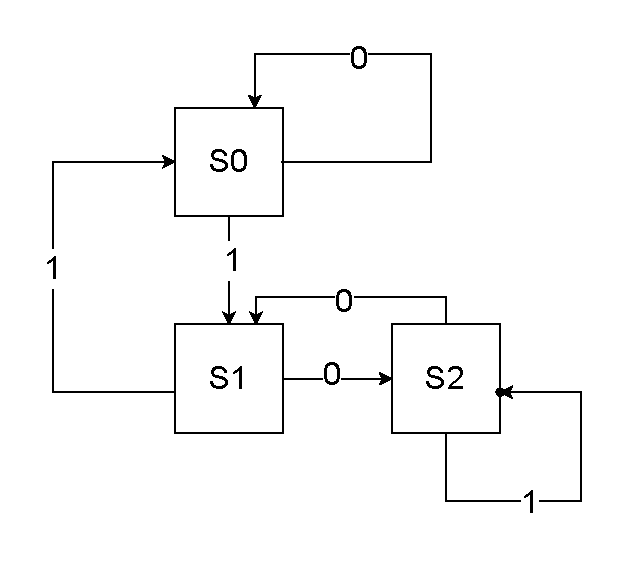
\includegraphics[width=0.7\textwidth]{pictures/DFA状态转移图.pdf}
	\caption{DFA状态转移图}
	\label{fig:DFA状态转移图}
\end{figure}
作者可以用这个状态转换图来实现一个简单的有限状态机,用于检测二进制数是否是 3 的倍数。
例如,考虑二进制数字 "110"(对应十进制的 6):
\begin{itemize}
	\item 初始状态:$ S_0 $
	\item 读取第一个字符 '1':状态从$ S_0 $变为$ S_1 $
	\item 读取第二个字符 '1':状态从$ S_1 $变为$ S_0 $
	\item 读取第三个字符 '0':状态从$ S_0 $变为$ S_0 $
\end{itemize}
最终状态是$ S_0 $,因此 "110" 是 3 的倍数。

\subsection{确定有限状态自动机}
确定性有限状态机(Deterministic Finite State Machine,DFA)是自动机的一种常见类型。
DFA具有以下几个特征和工作原理:
\begin{enumerate}
	\item 确定性转移: 对于给定的输入符号和当前状态,在DFA中每个状态只对应一个确定的下一个状态。
 也就是说,对于任何时刻,DFA可以根据当前状态和输入符号直接确定下一个状态,没有歧义或多义性。
	\item 状态转移: DFA通过状态转移来处理输入序列。从起始状态开始,根据输入符号,
 使用转移函数δ将DFA移动到下一个状态,然后继续接受下一个输入符号,如此往复,直到结束。
	\item 终止状态: 当DFA达到一个终止状态时,它表示DFA已经完成了特定的任务或接受了特定的输入序列。
 终止状态可以是一个或多个,DFA的任务和行为取决于达到哪些终止状态。
	\item 接受和拒绝: 执行结束后,如果DFA的最终状态属于终止状态集合F,则它接受输入序列;
 否则,它拒绝输入序列。
	\item 状态转移图: DFA的行为通常用状态转移图(State Transition Diagram)表示。
 状态用节点表示,转移用箭头表示。起始状态通常有一个入口箭头指向它,终止状态可能通过双圈或其他标记来表示。
\end{enumerate}
DFA是一种简单且易于理解的自动机模型。由于其确定性的特征,DFA在模式匹配、语法分析、词法分析和编译器设计等领域中得到广泛应用。
DFA可以用于验证、识别和处理各种类型的输入,如编程语言的关键字、标识符或语法规则等。它是构建更复杂自动机的基础,如正则表达式引擎和有限状态机网络。
\subsection{非确定有限状态自动机}
非确定性有限状态机(Nondeterministic Finite State Machine,NFA)是自动机的另一种常见类型,
与确定性有限状态机(DFA)相比,它具有一些特殊的特征和行为。

NFA具有以下几个特征和工作原理:
\begin{enumerate}
	\item 非确定性转移: 在NFA中,对于给定的输入符号和当前状态,一个状态可以对应多个可能的下一个状态。
 这样的非确定性转移使得NFA在处理输入时具有更大的灵活性。
	\item ε-转移(ε-Transition): NFA可以进行ε-转移,即在不消耗输入符号的情况下从一个状态跳转到另一个状态。
 这样的转移可以让NFA同时处于多个状态。
	\item 状态转移: 与DFA类似,NFA通过状态转移来处理输入序列。
 根据当前状态和输入符号,NFA使用转移函数δ将其移动到下一个状态集合。
	\item 终止状态: 当NFA中的任何一个状态达到终止状态时,它表示NFA已经完成了特定的任务或接受了特定的输入序列。
	\item 接受和拒绝: NFA根据其终止状态的集合来接受或拒绝输入序列。如果在执行结束时,
 NFA的最终状态中至少有一个状态属于终止状态集合F,则它接受输入序列;否则,它拒绝输入序列。
    \item 状态转移图: NFA的行为通常用状态转移图表示,其中状态用节点表示,转移用箭头表示。
    不同于DFA,NFA的转移箭头可以具有ε-转移和多个目标状态。
\end{enumerate}
NFA相比于DFA具有更大的灵活性和表达能力。由于其非确定性的特征,NFA在正则表达式引擎、模式匹配、语言处理和编译器设计等领域中得到广泛应用。
NFA通常被用作构建更复杂自动机模型的基础,如非确定性推导树和确定性有限状态机(DFA)。

本工具原型中,根据生成的AST,首先生成的只是相应的NFA,但是要想准确定位错误,能够将某一个状态具体对应到代码的某一段,还需要将NFA转换成
DFA,对于这一转换,本工具原型采用的是子集构造法。
\subsection{子集构造法}
子集构造法(Subset Construction Method)是一种将非确定有限状态自动机(NFA)转换为等价的确定有限状态自动机(DFA)的算法。
该算法的基本思想是根据NFA的状态集合构造DFA的状态集合,并在状态转移函数中处理相应的转移。

以下是子集构造法的大体步骤:
\begin{enumerate}
	\item  初始状态:
 从NFA的初始状态开始,构造DFA的初始状态,即将初始状态作为DFA的初始状态。
    \item  状态转移:
对于每个DFA状态和每个输入符号,找到对应的NFA状态集合。
对于该输入符号,将NFA状态集合进行ε-闭包处理,即找到所有通过ε(空转移)可以到达的状态。
将得到的ε-闭包状态集合作为DFA状态的转移目标,并根据输入符号找到相应的转移。
    \item  状态集合构建:
对于每个新构造的DFA状态,重复第二步骤,直到没有新的状态可以构造。
    \item  判断接受状态:
根据NFA的接受状态集合来判断DFA的接受状态。
如果DFA的状态集合中包含任何一个NFA的接受状态,则将该DFA状态标记为接受状态。
\end{enumerate}
通过使用子集构造法,可以将NFA转换为等价的DFA。


\section{抽象语法分析树}
抽象语法树(Abstract Syntax Tree,AST)是一个用于代表程序代码层次结构的树状数据结构。许多编译器,解释器以及静态分析工具都是以此为
开发基础。AST通过将代码语法拆解成了抽象的语法树结构,提供了一种以层次化,结构化理解和处理代码的方式。代码提示,格式化,debug工具,或者自动生成序列化代码等等,这些功能的开发都需要语法树里面的信息。
AST将代码中的各个元素(如表达式Expression,语句Statement,声明Declaration等)转化为语法树中的节点,而节点之间通过父子关系建立连接。
通常情况下,AST的根节点表示整个代码文件,然后每个语法结构(如函数、循环、条件语句等)都成为根节点的子节点。子节点可以继续有自己的子节点,以此类推,形成一个树状结构。

例如,对于一段表示欧几里得算法的C语言代码:\\
\begin{figure}[htbp]
    \centering
\begin{minipage}{4cm}
\begin{lstlisting}[language=c++]
while b ≠ 0:
    if a > b:
        a := a - b
    else:
        b := b - a
return a
\end{lstlisting}
\end{minipage}

\end{figure}


其AST的每一棵子树都会对应语句中的某一部分,
如while子树将会有condition和body两个子树,condition中包含了用于判断的表达式,body则是包含了判断为true时
需要执行的内容,如图\ref{fig:AST树}所示:
\begin{figure}[htbp]
	\centering
	\includegraphics[width=0.6\textwidth]{pictures/AST树.png}
	\caption{AST树}
	\label{fig:AST树}
\end{figure}


Clang的抽象语法树(AST)类层次结构主要分为以下几大类,每一类都代表不同的语言构造和抽象概念。

第一类是AST Context(AST上下文),它管理类型和声明的内存池。

第二类是Declaration(声明),代表各种声明,如变量声明、函数声明等。它的子类包括具名声明(NamedDecl),表示有名字的声明,如变量、函数、类型别名;和类型声明(TypeDecl),表示类、结构体、枚举等类型。具名声明的子类有值声明(ValueDecl),表示变量和函数等具有值的声明,以及类型声明(TypeDecl),表示类型别名和标签类型。模板声明(TemplateDecl)也属于这一类。

第三类是DeclContext(声明上下文),它是可以包含其他声明的上下文,如命名空间、记录、函数体等。命名空间声明(NamespaceDecl)和记录声明(RecordDecl)是DeclContext的子类。

第四类是Statement(语句),代表各种语句,如表达式语句、控制流语句等。它的子类包括表达式(Expr)、复合语句(CompoundStmt,表示包含多条语句的语句块)、if语句(IfStmt)、for循环语句(ForStmt)、while循环语句(WhileStmt)和return语句(ReturnStmt)。

最后一类是Type(类型),表示具体的数据类型,如int、char等。

在Clang生成的AST中,其根节点是TranslationUnitDecl,代表了一个C语言程序,可以从此开始遍历整个AST树,也可以获取已解析的的标识符表。
Clang的AST节点并没有一个共同的“NODE”基类,大部分AST节点派生自 Type、 Decl、 DeclContext 或Stmt,还有一些节点属于自己的特定结构。
因此,要遍历完整的AST,需要从TranslationUnitDecl开始,然后递归地遍历从该节点可以到达的所有内容,并针对每种特定节点类型对这一信息进行编码。
该算法被编码在一个RecursiveASTVisitor中。
\section{程序控制流图}
程序控制流图程序控制流图(Program Control Flow Graph)是一种用于表示程序执行流程的图形结构。
它描述了程序中不同语句之间的控制流结构。
程序控制流图有助于可视化和分析程序的结构,并在软件工程中广泛应用于代码分析、特别是数据流分析相关的技术。

一个程序控制流图由以下几个基本元素组成:
\begin{itemize}
	\item 基本块(Basic Block):基本块是程序控制流图的基本单元,它是一组语句的顺序执行序列。基本块内部没有分支和跳转语句,只有一个进入点和一个退出点。基本块可以包含多行代码,但通常被简化为单个语句。
    \item 控制边(Control Edge):控制边用于表示程序控制的转移关系。它连接了控制流图中的不同基本块,指示程序的执行流从一个基本块转移到另一个基本块。控制边也可以表示条件分支、循环结构和其他控制转移。
    \item 进入点(Entry Point):进入点是控制流图中的起始点,它标识程序的入口,表示程序开始执行的位置。
    \item 退出点(Exit Point):退出点是控制流图中的终止点,它标识程序的出口,表示程序结束执行的位置。
\end{itemize}

从AST生成CFG的过程涉及根据语法结构中的控制流语句
(如条件语句、循环语句等)来构建控制流。通过遍历AST树并识别程序流控制相关的节点,
工具原型可以建立一个CFG来表示程序中的控制流。

举个例子,考虑以下简单的代码片段,一个main函数中包含了一个while循环:\\

\begin{figure}[htbp]
    \centering
\begin{minipage}{4cm}
\begin{lstlisting}[language=c++]
int main() {
    int i = 0;
    while (i < 10) {
        i++;
    }
    return 0;
}
\end{lstlisting}
\end{minipage}
\end{figure}

首先,编译器或解析器会将这段代码转化为AST,如下图所示。

\begin{tikzpicture}
\Tree
[.TranslationUnit
    [.FunctionDeclaration(main)
        [.CompoundStatement
            [.VariableDeclaration ]
            [.WhileStatement 
                [.Condition ]
                [.CompoundStatement 
                    [.ExpressionStatement ]
                ]
            ]
            [.ReturnStatement ]
        ]
    ] 
]

\end{tikzpicture}
\begin{comment}
\begin{figure}[htbp]
	\centering
	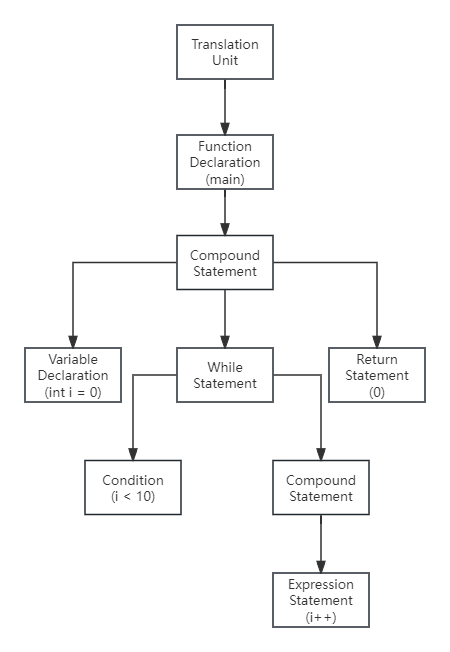
\includegraphics[width=0.5\textwidth]{pictures/AST例子.png}
	\caption{AST例子}
	\label{fig:AST例子}
\end{figure}
\end{comment}

然后,通过分析AST,工具原型可以构建一个简单的CFG来表示控制流,如图\ref{fig:cfg的例子}所示。





\begin{figure}[htbp]
	\centering
	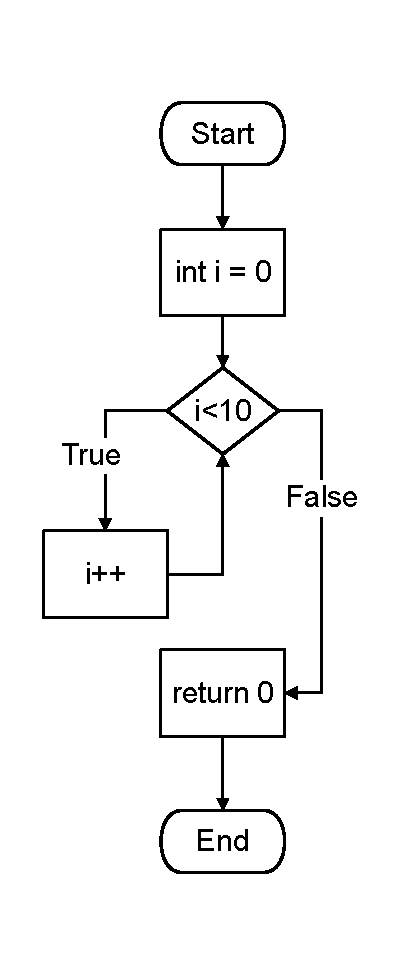
\includegraphics[width=0.3\textwidth]{pictures/cfg例子.pdf}
	\caption{cfg的例子}
	\label{fig:cfg的例子}
\end{figure}




值得注意的是,在本工具原型中,作者关注的主要是由日志函数,
所以,对于一些不包含日志的语句或者结构简单的语句,可以当作空语句处理
,这有助于简化CFG的整体结构。
\section{本章小结}
本章详细介绍了工具原型所运用的各类技术,包括 Clang 和 Libclang,用于生成和解析 C语言 程序的抽象语法树(AST),以及自动机(NFA 和 DFA)的基本概念及其在程序控制流图中的应用。最后,本文阐述了抽象语法树和程序控制流图的基本原理和结构。


\chapter{工具原型设计}
本章节描述了整个工具原型的功能需求和主要处理步骤的设计。论文所述工具原型的主要功能是为C语言程序
生成一个保留了日志记录信息的有穷自动机,然后使用这样的自动机来分析C语言程序运行时刻产生的日志记录,获取该C语言程序的运行时刻信息,支持对该类程序的排错和维护。
主要子功能包括从 C语言程序 生成抽象语法树,从语法树生成不确定的有穷自动机,获取NFA中调用日志记录函数的信息并生成确定的有穷自动机(DFA),
以及使用这类有穷自动机来分析日志记录并获得C语言程序运行时刻的信息。

\section{工具原型的功能和主要模块设计}
本工具原型主要有两大功能,即根据输入的C语言程序生成能够反映其日志记录过程的确定有穷状态自动机的功能,以及使用该有穷自动机对
C语言程序在运行时产生的日志记录进行分析以获得其运行时信息的功能。

第一个功能分成如图\ref{fig:系统流程图}所示的主要步骤:
\begin{enumerate}
	\item 使用Clang库扫描C语言程序,生成该程序对应的抽象语法树Clang-AST;
    \item 通过遍历AST,处理C语言程序中的各个函数定义,并对函数体中的语句进行递归处理,生成基本的不确定有穷自动机NFA;
    \item 对C语言程序中各个函数对应的NFA进行处理,包括消除掉无关的信息,处理函数调用,并保留日志记录函数调用的信息,生成有关日志函数的NFA;
    \item 使用子集构造法,将此NFA转换成为确定的有穷状态自动机DFA。
\end{enumerate}

根据上面的处理过程,本工具原型的主要模块主要包括:Clang扫描模块,NFA生成模块,NFA到DFA的转换模块,以及日志序列扫描分析模块。

\textbf{Clang扫描模块}的过程比较简单,它直接调用Clang的接口,将 C语言 源代码转化为抽象语法树 (AST),

在生成 AST 后,\textbf{NFA生成模块}从抽象语法树的根节点开始,遍历抽象语法树的所有节点,对其中的每个对应于C函数定义的AST节点进行处理,生成对应的 NFA。
每个NFA使用Automaton类的对象表示。为了使得这个模块能够具有更好的扩展性,将来可能用于其它目的的程序分析工具,这个对象中还记录了相应抽象语法树节点的信息、
对于这个初始NFA,\textbf{NFA生成模块}将进一步处理,过滤掉针对日志记录分析无用的转换标签,仅保留日志记录函数调用信息。
经过处理后,原来仅仅保护无用标签的边将被视作空边处理。

\textbf{NFA到DFA的转换模块}使用子集构造法,将带有日志记录的NFA转化为确定的有穷自动机DFA。该模块首先实现了对于NFA中的状态,返回其epsilon闭包(通过空边换可以到达的所有状态的集合)的函数,接着调用返回epsilon闭包的函数,在算法中“并行地模拟”NFA在遇到一个给定输入串
时可能执行的所有动作,最终构造得到的DFA的每个状态和NFA的状态子集对应。\\


第二个功能,\textbf{日志序列扫描分析模块}将待处理的日志序列作为上面构造的DFA的输入,通过追踪记录DFA识别过程中的状态转移序列来分析日志序列,获取C语言程序的运行状态信息。在此过程中,模块能够根据DFA的规则解析日志序列,验证其是否符合预期的模式。对于合法掉日志序列,该模块将返回一个包含经过的DFA状态的列表。
通过这些列表,工具原型可以分析出C语言程序运行时刻的行为和相关信息。


\begin{figure}[htbp]
	\centering
	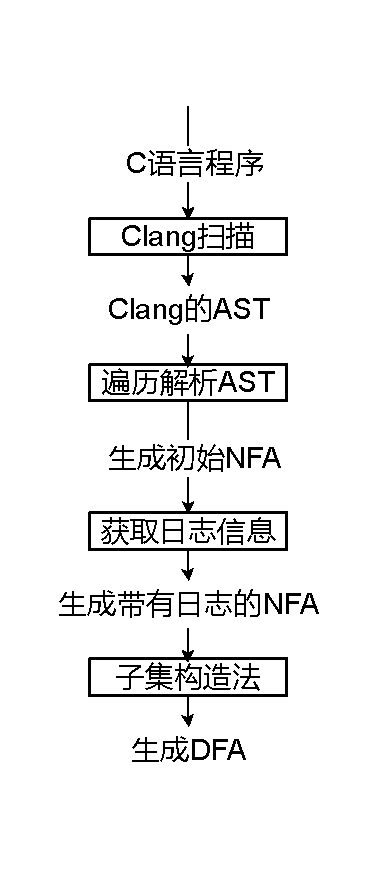
\includegraphics[width=0.25\textwidth]{pictures/系统流程图.pdf}
	\caption{系统流程图}
	\label{fig:系统流程图}
\end{figure}

\section{有穷自动机作为日志序列分析的基础}
一个系统在运行时会产生一系列的日志记录。这些日志在某种程度上记录了程序运行的历史,它也是系统维护和排错的重要依据。
程序员需要从日志记录中分析出尽可能多的系统运行信息,以提高维护和排错的效率。

因为效率的原因,系统通常只会记录关键事件的日志信息,导致从日志序列分析出系统运行信息变得相对困难。结合系统代码的信息,可以帮助人们从日志中分析得到更多的系统运行信息。
因此,本文使用有穷自动机对系统的源代码进行抽象描述,使之一方面能够反映源代码中的控制流信息,另一方面又能够高效处理日志记录序列。
首先对系统的源程序进行分析并生成有穷自动机,然后使用这个自动机高效地扫描输入的日志序列,
并根据扫描过程中经过的自动机的状态序列来获得更多的信息运行时刻信息。

源代码的控制流信息可以用有穷自动机来抽象地描述。
例如,对于程序中的每一条简单语句,可以直接使用一个简单的自动机来描述,形式为“状态1 -> 状态2”,其中状态1表示该语句的起始位置,状态2表示该语句的结束位置,而在转换的边上可以标注上这条语句的相关信息。而对于复杂语句,工具原型可以递归地为它的每个子语句生成相应的自动机。然后根据复杂语句的控制流结构,将子语句对应的自动机组合成为该复杂语句对应的自动机。诸如break、continue、return这样的控制流跳转语句,可以转换成为自动机状态之间的转换。
虽然这样构造的自动机忽略了很多源代码中的信息,但是它仍然能够在一定程度上反应出程序执行的控制流信息。

因为本文的目标是使用自动机来进行日志记录分析,因此源代码中对日志记录函数的调用被设置为自动机中相应转换的标号,而其它和日志记录无关的语句、表达式等被转换成为自动机中的$\epsilon$-转换。这个过程可以得到一个包含了程序的日志记录信息的不确定的有穷自动机。为了提高分析效率,本文将这个不确定有穷自动机转换成为确定的有穷自动机,并使用确定的有穷自动机高效地扫描和分析日志序列。
这样的处理使得自动机抽象地描述了程序的实际运行和日志记录情况。当自动机运行时,它会依据输入的条日志序列选择相应的边进行状态转换。
换句话说,这样的有穷自动机描述了日志生成的可能顺序,从而在一定程度上反映了程序的运行状态。

例如,如果系统的源程序有一条对日志记录函数的调用log("inside funcA"),表示程序执行到函数A内部。那么对应的自动机片段如图\ref{fig:日志函数对应的自动机片段}所示。

\begin{figure}[htbp]
	\centering
	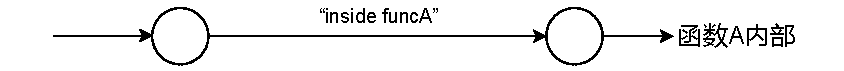
\includegraphics[width=1\textwidth]{pictures/函数调用示例.pdf}
	\caption{日志函数对应的自动机片段}
	\label{fig:日志函数对应的自动机片段}
\end{figure}
当程序执行中经过此语句时会向日志记录文件中插入一条"inside funcA"的日志记录。相应的,如果自动机分析日志记录文件中的日志序列时读入了"inside funcA", 它就能够判断系统程序在当时执行了语句log("inside fucA"),也就能判断出当时系统程序正在执行函数funcA。结合整个日志序列中的其它日志记录,就可以更加精确地分析出系统运行的信息。


\section{数据结构设计}
工具原型中主要有两类数据结构:一类是记录自动机信息的数据结构 Automaton,另一类是管理源程序的所有有穷自动机的数据结构 AutomatonManager。


\subsubsection{记录自动机信息的数据结构}
\begin{figure}[htbp]
	\centering
	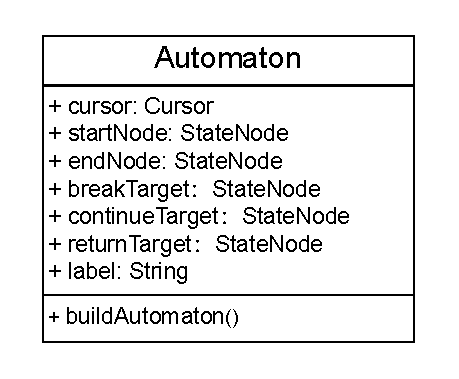
\includegraphics[width=0.5\textwidth]{pictures/Automaton的数据结构.pdf}
	\caption{Automaton的数据结构}
	\label{fig:Automaton的数据结构}
\end{figure}


Automaton类的对象记录了AST结点对应的自动机入口和出口和其他自动机的相关信息。
它的成员变量和方法如图\ref{fig:Automaton的数据结构}所示。

Automaton类的对象存有代表start和end的StateNode。StateNode类的对象代表了自动机的状态,它存有一个唯一的id,用于区分不同的状态。
其中Cursor类的对象cursor指向了相应的AST树结点,可以简单的将其看作对AST节点的“引用”。
此外,Automaton类的对象中还存有break语句,continue语句和return语句的跳转目标,它们以stateNode的形式表示,当下一层次的语句中存在
跳转语句时,便可将跳转语句的出口连接到相应的跳转目标上。
最后Automaton类的对象以字符串的形式储存了一个标签,用于表示边“startNode-->endNode”上的标签。

Automaton类中实现了buildAutomaton方法,当调用此方法时,如果对象为复杂语句,
会为当前语句的下一层次的语句生成相应的自动机片段,形成代表复杂语句的自动机层次结构,并将相关信息记录到Automaton类的对象;如果对象为简单语句,则不做处理。

对于简单语句,工具原型生成一个Automaton类的对象,它具有startNode和endNode两个state节点,并且有一条边从startNode连到endNode。

对于复杂语句,工具原型将生成一个Automaton类的对象,然后调用Automaton的方buildAutomaton,
这将为该语句的下一层次的语句也生成Automaton类的对象,从而递归地生成该复杂语句的自动机结构。

对于日志函数,工具原型同样地生成一个Automaton类的对象,其中边上的标签为日志函数“log”的输入参数。




\subsubsection{管理所有有穷自动机的数据结构}
\begin{figure}[htbp]
	\centering
	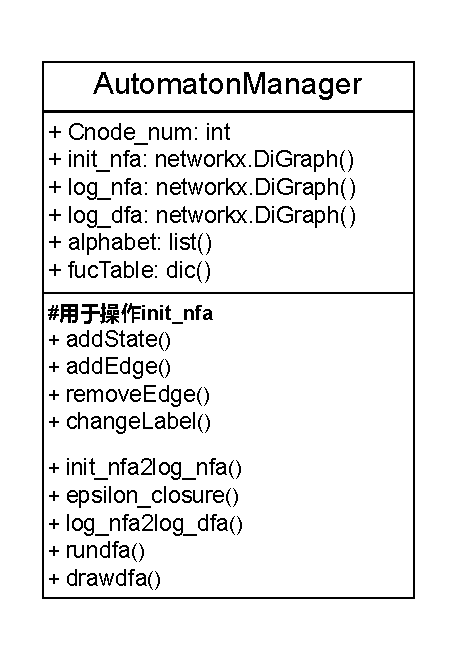
\includegraphics[width=0.5\textwidth]{pictures/AutomatonManager的数据结构.pdf}
	\caption{AutomatonManager的数据结构}
	\label{fig:AutomatonManager的数据结构}
\end{figure}
如图\ref{fig:AutomatonManager的数据结构},AutomatonManager类的对象以有向图的形式维护了所有生成的Automaton类的对象的连接信息,并实现了不同类型的图之间的转换方法。

AutomatonManager类的对象管理了所有生成的自动机,并将它们整合成一个代表C语言程序的自动机,其底层的数据结构是NetworkX库\cite{networkx}中的DiGraph类,它提供了一个易于维护的有向图结构,有向图中的节点代表自动机的状态,连边代表自动机的转移,边上的标签代表转移的输入字符。

AutomatonManager类的对象中有三个DiGraph类的对象:init\_nfa, log\_nfa和 log\_dfa,代表了工具原型运行到不同阶段时,代表C语言程序的不同类型的自动机。
\begin{itemize}
    \item  init\_nfa代表从AST树转换得到的非确定的有穷自动机。AutomatonManager类提供了修改该NFA的方法,可用于对自动机的图结构进行操作。如 addState() 可向init\_nfa中添加代表状态节点;addEdge(),removeEdge()可用于向init\_nfa中添加或者移除边;changeLabel()可用于添加或修改边上的标签。
自动机边的标签。
    \item  log\_nfa是在init\_nfa的基础上,删除掉无关信息,仅保留日志记录作为输入字符的非确定的有穷自动机。
    \item  log\_dfa则是根据 log\_nfa,利用子集构造法生成相应的确定的有穷自动机,其中一个DFA状态代表了一个NFA的状态集合。
\end{itemize}

除了维护自动机的图结构,AutomatonManager类还存有一个列表类型(list)的alphabet对象,用于储存所有日志函数的参数,作为自动机的合法输入字符集合。

最后,在处理 AST 中的函数调用节点时,AutomatonManager 类维护一个字典类型(dict)的 fucTable,用于将函数名映射到相应的 Automaton 对象。每当工具原型遇到函数调用节点时,会在 fucTable 中查找与该函数名对应的 Automaton 对象,并将该对象所记录的自动机连接到函数调用的位置。这种映射机制确保了函数调用的行为能够被精确地解析和执行。\\

AutomatonManager类还实现了不同自动机的图结构的转换方法,以及通过工具原型生成的DFA解析日志记录文件的方法。

首先,AutomatonManager类中实现了根据init\_nfa,生成带有日志函数的非确定有穷自动机  log\_nfa的方法:init\_nfa2 log\_nfa。它去除init\_nfa的有向图结构中的所有与日志函数无关的标签,使得所有日志函数的参数成为  log\_nfa 中的输入字符集合。

接着,该类实现了从非确定有穷自动机到确定的有穷自动机的转换方法  log\_nfa2 log\_dfa。它根据子集构造法,将  log\_nfa 进行转换,并存在 log\_dfa中。

最后,该类实现了一个根据已有的确定有穷自动机来解析日志的方法 rundfa。它以日志记录文件作为为输入序列,运行得到的DFA,并根据运行结果给出相应的分析:如日志合法性,C语言程序发生错误前的运行过程等。
\section{本章小结}
本章首先介绍了工具原型的功能,包括利用Clang生成抽象语法树,
根据AST生成NFA和DFA,以及使用DFA进行日志解析等功能。

然后描述了工具原型的模块设计,并对每个模块进行了解释。

接下来,文章围绕程序与自动机的对应关系展开了论述,解释了工具原型选择用NFA解析日志序列的原因。

最后,文章介绍了工具原型中需要的数据结构,
包括代表自动机的Automaton类以及管理了所有生成的自动机的AutomatonManager类,并介绍了这些类所实现的方法。




\chapter{工具原型实现}
本章描述了工具原型的一些关键功能的实现技术,主要包括如何利用Clang库来生成抽象语法树,以及根据抽象语法树来生生成输入程序对应的自动机。最好还描述了如何利用自动机进行日志定位。


\section{工具原型运行环境}
本工具原型使用Python语言实现。因此首先需要安装 Python 3.10.8\cite{python310} 版本的开发和运行此环境。
同时需要安装 Clang 12.0.0\cite{Clang12}库,供工具原型用于生成输入程序的抽象语法树。
安装 Clang库后,通过配置 PYTHONPATH 环境变量使其指向 Clang 的 Python 绑定模块 Clang.cindex,使得Python可以找到并使用 Clang 的相关功能。
同时还需要安装名为NetworkX\cite{networkx}的Python库。该库被用于一个用于创建和操作复杂网络的数据结构。

\section{关键功能实现}
本工具原型的关键功能包括如下几个部分:
\begin{enumerate}
    \item 使用Clang的Python库,将C语言程序转换为相应的抽象语法树;
    \item 递归地解析抽象语法树,生成相应的不确定有穷自动机(NFA);
    \item 从不确定有穷自动机出发,从中抽象掉无关信息,仅仅保留日志记录代码的信息,生成确定有穷状态自动机(DFA);
    \item 利用上述的DFA来解析日志序列,获取程序运行信息。
\end{enumerate}
在本小节中将逐个描述这些功能的实现方法。

\subsection{从C语言程序到AST树的转换方法}
对于给定的C语言待分析文件,
工具原型调用cindex模块生成并获取其AST。
其中cindex模块提供了Clang索引库的接口,如章节2.1所言,这个接口用Python封装了
Clang的C语言API,它能使工具原型用与C语言API相似的方式调用Clang来解析源文件。

图\ref{生成C语言程序的AST}的代码用于处理输入文件,生成Clang-AST\\
\begin{figure}[ht]
\centering
\begin{minipage}{12cm}
\begin{lstlisting}
index = cx.Index.create(excludeDecls=True)
tu = index.parse('main.cpp', args=['-std=c'])
pprint(("diags", [get_diag_info(d) for d in tu.diagnostics]))
\end{lstlisting}
\end{minipage}
\caption{生成C语言程序的AST}
\label{生成C语言程序的AST}
\end{figure}

首先工具原型创建了一个类型为Index的对象,该对象提供了cindex模块的主接口,
其主要作用是提供读取和解析翻译单元的接口,并
设置参数 excludeDecls=True,告诉Clang在索引中排除不需要的声明。
这可以减少内存使用并提高性能。

其次,工具原型使用Clang的解析器来解析C语言程序,这将调用Index的parse方法,
从给定的源代码文件加载翻译单元,
并返回一个TranslationUnit对象(tu),其中翻译单元是生成的AST树的根节点。
tu代表了解析源文件的翻译单元,其中 args=['-std=c']参数
指定了使用C语言标准进行解析,
这意味着代码将根据C语言标准的特性和规则进行分析。

最后,工具原型将调用tu中的diagnostics方法,这将返回一个在解析翻译单元时生成的诊断信息列表。
这些诊断信息可以包括错误、警告和信息提示。

\subsection{从根节点解析AST,生成初步的NFA的方法}
当得到了Clang生成的翻译单元,也就是AST树的根节点后,工具原型将从根节点遍历所有的AST节点
,找到每一个代表函数定义的节点。

所以用图\ref{递归遍历AST树,寻找所有的函数定义}所示的递归过程,从AST树的根结点出发,可以递归遍历整个AST树,找到所有函数定义,并对每个函数定义的AST结点生成相应的自动机(Automaton类的对象)。\\

\begin{figure}[ht]
\centering
\begin{minipage}{10cm}
\begin{lstlisting}
traverse(Cursor):
    if 节点类型 是 FUNCTION_DECL:
        if 节点 is 函数定义:
            记录函数出口,入口
            生成该函数节点的自动机(Automaton类)

    # 遍历下一层次的节点
    对当前AST节点的每个下一层次的节点:
        递归调用traverse

\end{lstlisting}
\end{minipage}
\caption{递归遍历AST树,寻找所有的函数定义}
\label{递归遍历AST树,寻找所有的函数定义}
\end{figure}

首先,程序接受一个AST节点的指针(cindex.Cursor)作为参数。在首次调用此递归函数时,该AST节点为上一步生成的翻译单元(TranslationUnit)。

然后,工具原型便判断该节点的类型是否为FUNCTION\_DECL且
节点代表的语句为函数定义,如果是,则提取该函数定义的函数体,
并构造自动机;反之则不做处理。
同时,工具原型还要维护Graph类中的map类数据结构,将得到的函数名和入口出口存入其中。

最后,工具原型将以所有下一层次的AST节点为输入参数,分别调用traverse函数,以达到递归遍历的效果。\\


对于代表语句的ASTNode,工具原型会生成一个对应的代表自动机的Automaton类的对象。

Automaton类的对象中储存了一个指向AST节点所代表的ASTNode的对象,AST节点的类型kind,
语句起始处的stateNode和语句终止处的endNode,以及两个stateNode之间的连接上的标签,标签的内容代表了AST节点代表的语句的类型。
它还包含了传入的跳转目标breakTgt,continueTgt和returnTgt,其中每一个target都是一个stateNode的对象。\\

下面,作者将结合代码,对生成自动机(如图\ref{Auto类的初始化})这一过程进行详细的介绍:

对于一个待生成自动机的AST节点,工具原型会首先初始化一个Automaton类的对象,
代表一个自动机。
Automaton类对象的初始化过程为即将执行的自动机构造过程设置了一些初始值和相关的参数,包括自动机的开始状态和结束状态,以及该AST结点对应的语句中包含的break、continue、return语句的跳转目标信息。\\
\begin{figure}[ht]
\centering
\begin{minipage}{12cm}
\begin{lstlisting}
__init__(cursor: Cursor,breakTgt,continueTgt):
    self.cursor = cursor
    设置break,continue和return的跳转目标
    为stateNode和endNode生成start和end状态
    ...
\end{lstlisting}
\end{minipage}
\caption{Auto类的初始化}
\label{Auto类的初始化}
\end{figure}

大多数情况下,如果AST节点并不需要工具原型提供跳转目标,当工具原型想要为该AST节点创建一个自动机(Automaton类)时,只需要把相应的AST节点自身传入init函数即可。
但是,当AST节点需要工具原型提供跳转目标时,
为了能正确的表示有关跳转的控制流信息,工具原型应该保证生成的自动机能够表示程序运行时可能的执行序列,
所以,工具原型将为需要的AST节点提供return,break和continue语句所需的三个跳转目标,也就是三个stateNode,具体实现如下:
\begin{itemize}
    \item 对于return语句的跳转目标,工具原型需要判断当前AST节点是否为函数体,
若为函数体,则将returnTgt设置为当前AST节点的endNode,
若不是函数体,则继承上一层次的AST节点生成的Automaton类对象中的returnTgt。
    \item 对于break,continue语句,因为代表它们跳转目标的stateNode是在上一层次的AST节点中,
而这些跳转目标,对于break,continue语句在初始化自动机时是未知的,所以工具原型还需要
在生成上一层次的AST节点(如for,while节点)的自动机时,正确传入相应的跳转目标,
然后等到生成下一层次的自动机时,再将其中需要跳转目标的自动机连接到相应的跳转目标(breakTgt或continueTgt)上。具体的说,上一层次的节点在调用buildAutomaton后改变了breakTgt或continueTgt,则会将新的跳转目标传入下一层次的节点;反之,下一层次的节点则直接继承上一层次节点的跳转目标。
\end{itemize}

最后,初始化函数会生成两个初始state,作为自动机的入口状态和出口状态。\\


当AST节点对应的初始化完成后,对于复杂语句,工具原型还需要进一步
根据节点类型,生成该自动机的内部层次结构。具体的说,就是生成下一层次的AST节点的
的自动机,并处理好它们之间的层次关系。
所以,在Automaton类对象初始化之后,还需要调用buildAutomaton方法。\\

图\ref{生成下一层次的AST节点的自动机}是Automaton类的方法 buildAutomaton,它将会根据AST节点类型,生成下一层次的AST节点的自动机,
并最终生成该自动机的内部层次结构。其中breakTgt,continueTgt等信息,均记录在对象self的成员变量中,可供buildAutomaton使用。
\\
\begin{figure}[ht]
\centering
\begin{minipage}{10cm}
\begin{lstlisting}
buildAutomaton(breakTgt,continueTgt): 
    获取下一层次的节点的列表 cursorChilds
    #对各种节点类型的判断及处理
    ...
    elif self.cursor.kind == CursorKind.COMPOUND_STMT:
    ... ...
    elif self.cursor.kind == CursorKind.FOR_STMT:
    ... ...
    elif self.cursor.kind == CursorKind.WHILE_STMT:
    ... ...
    elif self.cursor.kind == CursorKind.IF_STMT:
    ... ...
    elif self.cursor.kind == CursorKind.SWITCH_STMT:
    ...
    
\end{lstlisting}
\end{minipage}
\caption{生成下一层次的AST节点的自动机}
\label{生成下一层次的AST节点的自动机}
\end{figure}

对于整个AST的分析,都建立在递归调用buildAutomaton上的,当某一个Automaton类对象调用该函数时,它便会生成该对象的下一层次所有节点的Automaton类的对象,具体步骤为:
\begin{enumerate}
	\item 判断该AST节点的类型,并获取下一层次的AST节点。
	\item 调用每个下一层次的AST节点的buildAutomaton方法,递归生成下一层次的节点的自动机结构。
	\item 根据节点类型,处理下一层次的AST节点之间的层次关系,并以这种更细致的层次结构重新连接 start\_state-->end\_state

\end{enumerate}

递归调用buildAutomaton,从而生成自动机的过程,是整个工具原型中的重要环节。
下面将对buildAutomaton方法中,关于各种类型的AST节点的处理进行详细解释。

\subsubsection{对break,continue和return语句的处理}
图\ref{跳转语句处理}是对break,continue和return节点的处理的伪代码。因为程序的控制流会在
这些语句发生跳转,所以,工具原型需要将AST节点对应的自动机连接到跳转目标上,
其中每一个跳转目标都是一个stateNode类的对象。

\begin{figure}[ht]
\centering
\begin{minipage}{12cm}
\begin{lstlisting}
buildAutomaton(breakTgt,continueTgt): 
    if self.cursor.kind == CursorKind.BREAK_STMT:            
        从break自动机的endNode连接到已传入的breakTgt
    elif self.cursor.kind == CursorKind.CONTINUE_STMT:
        从continue自动机的endNode连接到已传入的continueTgt
    elif self.cursor.kind == CursorKind.RETURN_STMT:
        从return自动机的endNode连接到已传入的returnTgt
\end{lstlisting}
\end{minipage}
    \caption{跳转语句处理}
    \label{跳转语句处理}
\end{figure}

因为工具原型在生成这些跳转语句的上层次节点的自动机时,已经分配好了跳转目标,所以在这里工具原型只需将跳转语句的自动机连接到
已经传入的跳转目标上即可。

\begin{comment}
\subsubsection{对表达式语句的处理}
图\ref{表达式处理}是对表达式的节点的处理的伪代码。

\begin{figure}[ht]
\centering
\begin{minipage}{10cm}
\begin{lstlisting}
buildAutomaton(breakTgt,continueTgt): 
    elif self.cursor.kind == CursorKind.DECL_STMT:
        ...
    elif self.cursor.kind == CursorKind.BINARY_OPERATOR:
        ...
    elif self.cursor.kind == CursorKind.UNARY_OPERATOR:
        ...
\end{lstlisting}
\end{minipage}
    \caption{表达式处理}
    \label{表达式处理}
\end{figure}
\end{comment}


表达式代表的AST节点均为简单的结构,所以工具原型只是为其添加了标签,方便展示中间结果。

\subsubsection{对函数调用的处理}
图\ref{函数调用处理}是对函数调用的节点的处理的伪代码,工具原型用不同方式处理了日志函数和其他普通的函数。

\begin{figure}[ht]
\centering
\begin{minipage}{9cm}
\begin{lstlisting}
buildAutomaton(breakTgt,continueTgt): 
    elif self.cursor.kind == CursorKind.CALL_EXPR:
        if 函数名为"log":
            对日志函数的处理
        else:
            对普通函数调用的处理
\end{lstlisting}
\end{minipage}
    \caption{函数调用处理}
    \label{函数调用处理}
\end{figure}

当AST节点是一般函数的调用时,工具原型需要先来到到储存函数表的map中,查找对应函数的入口和出口,
并将函数的入口和出口连接到函数调用的位置所在的上文和下文。

当AST节点是log日志函数的调用时,工具原型获取log函数的参数,并将其添加到自动机的输入字
符集中,最后将参数作为标签,添加到边上。

\subsubsection{对顺序结构(复合语句)的处理}
图\ref{顺序结构处理}是对顺序结构的处理的伪代码,这将生成所有下一层次的节点的自动机并按照顺序连接。\\
\begin{figure}[ht]
\centering
\begin{minipage}{14cm}
\begin{lstlisting}
buildAutomaton(breakTgt,continueTgt): 
    elif self.cursor.kind == CursorKind.COMPOUND_STMT:
        对于下一层次的的每一个节点:  
            生成下一层次的节点的Automaton类的对象
            以从后往前的顺序,连接每一个下一层次的节点的Automaton类的对象
\end{lstlisting}
\end{minipage}
    \caption{顺序结构处理}
    \label{顺序结构处理}
\end{figure}

顺序结构会以类型为compound statement(复合语句)的AST节点存在,生成到源程序的AST树上。对于这类AST节点,
它的下一层次的AST节点生成的自动机需要按照顺序依次连接,最后连复合语句回该节点生成的自动机。

\begin{figure}[htbp]
	\centering
	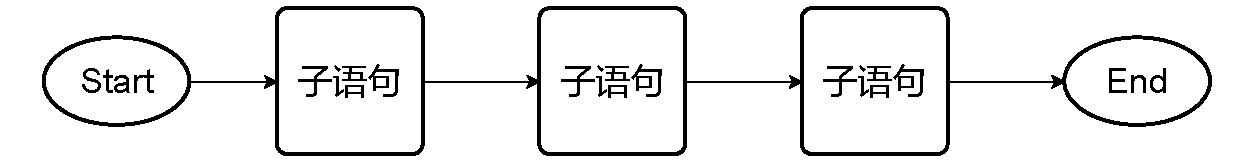
\includegraphics[width=1\textwidth]{pictures/顺序结构.pdf}
	\caption{顺序结构}
	\label{fig:顺序结构}
\end{figure}

图\ref{fig:顺序结构}是顺序结构的程序控制流图。
当复合语句中存在跳转语句时,工具原型需要正确提供跳转目标,但是如果正常地从前往后生成,便可能
出现跳转目标还未生成,工具原型无法提供的情况,所以工具原型在实现上选择了反向连接,如此便保证了所有跳转目标都能在被需要之前生成。


\subsubsection{对for结构的处理}

 \begin{figure}[htbp]
	\centering
	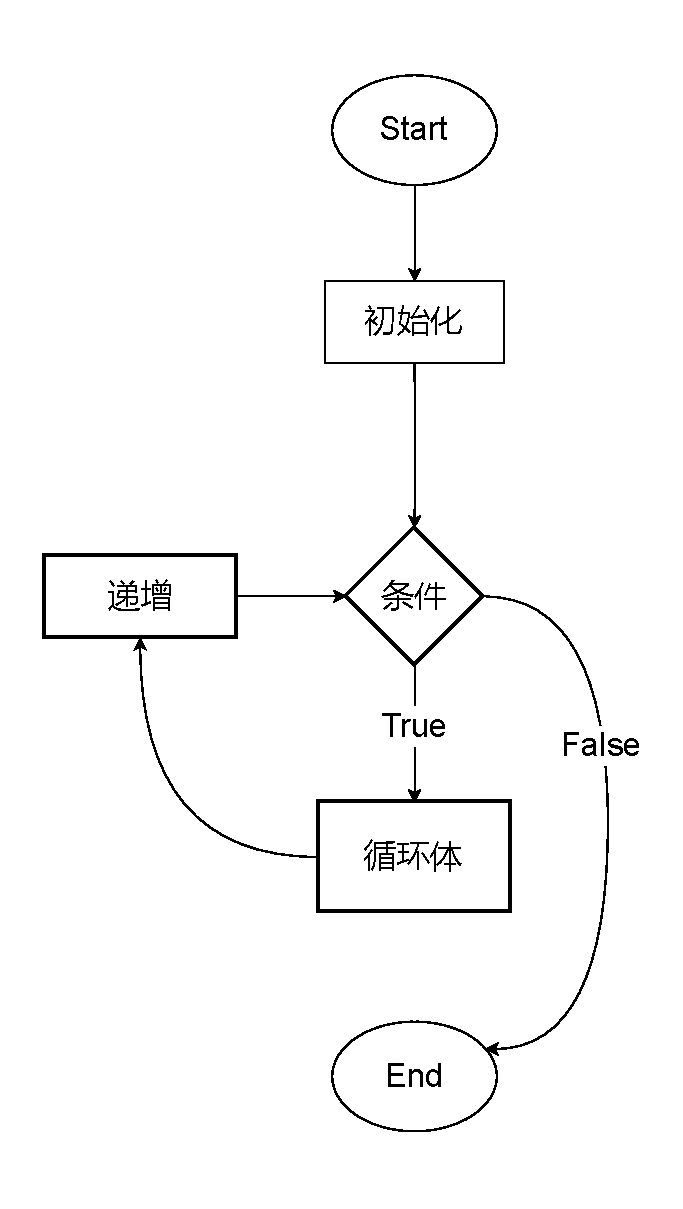
\includegraphics[width=0.4\textwidth]{pictures/for结构.pdf}
	\caption{for的控制流图}
	\label{fig:for的控制流图}
\end{figure}

图\ref{fig:for的控制流图}是for语句的程序控制流图,其中for语句的初始化语句,条件语句,递增语句均有可能为空。
根据C语言的语义,for语句首先执行初始化语句,接着计算条件语句。如果条件表达式为假,则for语句执行结束;如果条件表达式的值为真,那么继续执行循环体中的语句。循环体执行完毕后,程序将执行递增语句,最后返回到条件表达式的开始处继续执行。

for语句中的break和continue语句需要特殊处理:循环体中的break语句执行之后将结束for语句的执行;而continue语句执行之后,程序将转到条件语句处继续执行。即
工具原型在循环体内部处理 break 语句时,需要将该 break 语句对应的
自动机的出口连接到for语句自动机的出口; 在处理 continue 语句时,需要将 continue 语句的自动机的出口连接
到连接到条件语句自动机的入口。\\

\begin{figure}[ht]
\centering
\begin{minipage}{16cm}
\begin{lstlisting}[language=Python]
buildAutomaton(breakTgt,continueTgt): 
    解析for节点,获取该节点的下一层次的节点存在与否的情况。
    根据解析结果,分别生成下一层次的节点的自动机或者代表空节点的自动机:
        获取init的AST节点cond,并构造生成init的自动机initAutomaton
        获取condition的AST节点cond,并构造生成condition的自动机condAutomaton
        获取increasement的AST节点incAutomaton,并构造生成increasement的自动机incAutomaton
    获取statements的AST节点stmts
    stmtsAutomaton = Automaton()        #为循环体初始化一个Automaton类的对象
    stmtsAutomaton.buildAutomaton(stmts,breakTgt=self.end_state,continueTgt=condAutomaton.start_state)     
    #构造statements的自动机stmtsAutomaton
    按照程序控制流图,将for语句中不同部分的自动机连接起来
\end{lstlisting}
    \caption{for结构处理}
    \label{for结构处理}
\end{minipage}
\end{figure}


图\ref{for结构处理}是对for类型节点的处理的伪代码。
工具原型首先判断下一层次中init,condition,increasement三个位置的AST节点的存在与否,生成初始化init的自动机initAutomaton,条件表达式cond的自动机condAutomaton和递增语句的自动机incAutomaton:
\begin{itemize}
    \item 对于存在的AST节点,工具原型将先获取所在位置的AST节点接着,工具原型将为该AST节点初始化一个Automaton类的对象,生成它的自动机。
    \item 对于不存在的AST节点,工具原型将专门初始化一个类型为“empty”的空节点的自动机,用于填充空缺的节点,保持for语句的自动机原有的层次结构。
\end{itemize}

下一步,工具原型将先获取for语句中的statements的AST节点stmts。然后为stmts初始化一个Automaton类的对象stmtsAutomaton.
因为 for 语句的循环体中的 break 将中止 for 语句的执行,工具原型应该将for语句的endNode作为循环体中的break语句的跳转目标(breakTgt)。
同样的,因为 for 语句的循环体中的continue将开始下一轮的循环,工具原型应该将条件表达式对应的NFA的startNode作为循环体中的continue语句的跳转目标(continueTgt)。



最后调用buildAutomaton方法递归生成stmtsAutomaton的不确定自动机。并按照程序控制流图,将for语句中不同部分的自动机连接起来:
\begin{itemize}
    \item for语句的自动机的入口连接到initAutomaton的入口;
    \item initAutomaton的出口连接到condAutomaton的入口;
    \item condAutomaton的出口将以“True”的标签连接到stmtsAutomaton的入口,同时以“False”的标签连接到for语句的自动机的入口;
    \item stmtsAutomaton的出口将连接上incAutomaton的入口;
    \item incAutomaton的出口将连接上condAutomaton的入口。
\end{itemize}



\subsubsection{对while结构的处理}
 \begin{figure}[htbp]
	\centering
	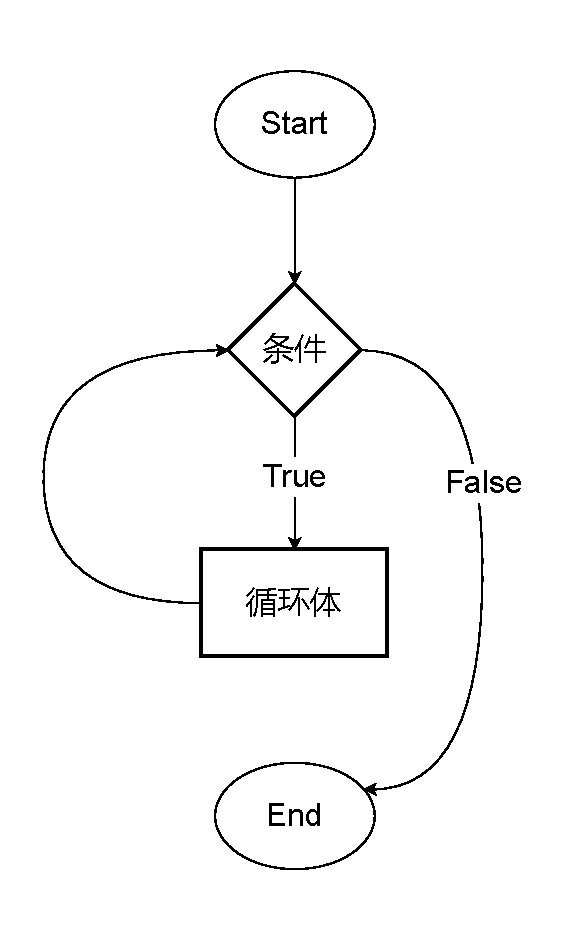
\includegraphics[width=0.4\textwidth]{pictures/while结构.pdf}
	\caption{while的控制流图}
	\label{fig:while结构}
\end{figure}

图\ref{fig:while结构}是while语句的程序控制流图。
根据C语言的语义,while语句首先计算条件语句。如果条件表达式为假,则while语句执行结束;如果条件表达式的值为真,那么继续执行循环体中的语句。循环体执行完毕后,程序将返回到条件表达式的开始处继续执行。

while语句中的break和continue语句需要特殊处理:循环体中的break语句执行之后将结束while语句的执行;而continue语句执行之后,程序将转到条件语句处继续执行。即
工具原型在循环体内部处理 break 语句时,需要将该 break 语句对应的
自动机的出口连接到while语句自动机的出口; 在处理 continue 语句时,需要将 continue 语句的自动机的出口连接
到连接到条件表达式自动机的入口。\\

\begin{figure}[ht]
	\centering
\begin{minipage}{16cm}
\begin{lstlisting}
buildAutomaton(breakTgt,continueTgt): 
    获取condition的AST节点cond,并构造生成condition的自动机condAutomaton
    获取statements的AST节点stmts
    stmtsAutomaton = Automaton()        #为循环体初始化一个Automaton类的对象
    stmtsAutomaton.buildAutomaton(stmts,breakTgt=self.end_state,continueTgt=condAutomaton.start_state)     
    #构造statements的自动机stmtsAutomaton
    按照程序控制流图,将while语句中不同部分的自动机连接起来
\end{lstlisting}
\end{minipage}
    \caption{while语句的处理}
    \label{while结构处理}
\end{figure}

图\ref{while结构处理}是对while语句处理的伪代码,其中while语句的条件节点必定不为空。
工具原型将先获取while语句中的condition的AST节点cond和statements的AST节点stmts。然后为条件表达式cond生成自动机condAutomaton(它是Automaton类的一个对象).

下一步,工具原型将先获取while语句中的statements的AST节点stmts。然后为stmts初始化一个Automaton类的对象stmtsAutomaton.
因为 while 语句的循环体中的 break 将中止 while 语句的执行,工具原型应该将while语句的endNode作为循环体中的break语句的跳转目标(breakTgt)
同样的,因为 while 语句的循环体中的continue将开始下一轮的循环,工具原型应该将条件表达式对应的NFA的startNode作为循环体中的continue语句的跳转目标(continueTgt)。

最后按照程序控制流图,将while语句中不同部分的自动机连接起来:
\begin{itemize}
    \item while语句的自动机的入口连接到condAutomaton的入口;
    \item condAutomaton的出口将以“True”的标签连接到stmtsAutomaton的入口,同时以“False”的标签连接到while语句的自动机的入口;
    \item stmtsAutomaton的出口将连接上condAutomaton的入口。
\end{itemize}

\subsubsection{对if结构的处理}

 \begin{figure}[htbp]
	\centering
	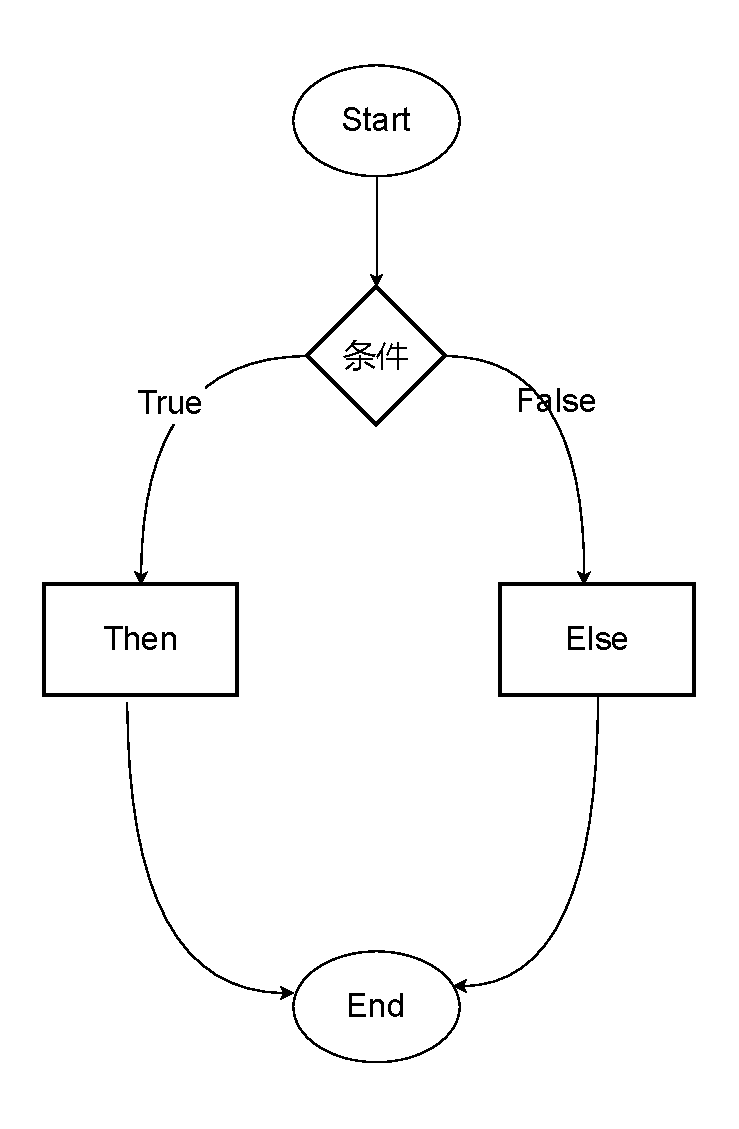
\includegraphics[width=0.4\textwidth]{pictures/if结构.pdf}
	\caption{if的控制流图}
	\label{fig:if的控制流图}
\end{figure}

图\ref{fig:if的控制流图}是if语句的程序控制流图。
根据 C语言 的语义,if语句首先计算条件语句。如果条件表达式为假,
则 执行if语句中的then分支;如果条件表达式的
值为真,那么继续执行执行if语句中的else分支。

if 语句中的 break 和 continue 语句不需要特殊处理。
在为 if 语句中的then分支和else分支生成 NFA 时,工具原型应该将 if 语句上一层次的语句自动机中记录的跳转目标(breakTgt,continueTgt)直接继承给if 语句中的then分支和else分支,作为 if 语句中的then分支和else分支 break语句和continue语句的跳转目标。即工具原型在then分支和else分支内部处理 break和continue 语句时,需要将该 break 语句对应的自动机的出口连接到上一层次的语句自动机的breakTgt和continueTgt.

\begin{figure}[ht]
	\centering
\begin{minipage}{16cm}
\begin{lstlisting}
buildAutomaton(breakTgt,continueTgt): 
    获取condition的AST节点cond,并构造生成condition的自动机condAutomaton
    获取then分支的AST节点then-branch
    thenAutomaton = Automaton(); #为then-branch初始化一个Automaton类的对象
    thenAutomaton.buildAutomaton(then,breakTgt=self.breakTgt,continueTgt=self.continueTgt)    
    #构造statements的自动机stmtsAutomaton
    if 该ASTNode代表一个带有else分支的if语句:
        获取else分支的AST节点else-branch
        elseAutomaton = Automaton(); #为else-branch初始化一个Automaton类的对象
        elseAutomaton.buildAutomaton(else,breakTgt=self.breakTgt,continueTgt=self.continueTgt)    
        #构造else的自动机elseAutomaton
        按照程序控制流图,将if语句中不同部分的自动机连接起来
    else:
        按照程序控制流图,将没有else分支的if语句中不同部分的自动机连接起来
\end{lstlisting}
\end{minipage}
    \caption{if结构处理}
    \label{if结构处理}
\end{figure}

图\ref{if结构处理}是对if结构的处理的伪代码。
工具原型将先获取if语句中的condition的AST节点cond和then分支的AST节点then。
然后为条件表达式 cond 生成自动机 condAutomaton(它是 Automaton 类的一个
对象);同时为 then 初始化一个 Automaton 类的对象 thenAutomaton,继承if自动机本身的breakTgt和continueTgt,
最后调用 buildAutomaton 方法递归生成 thenAutomaton 的不确定自动机。

下一步,工具原型对if的AST节点的下一层次节点中有else分支和没有else分支的两种情况做出不同的处理,最后按照程序控制流图,将if语句中不同部分的自动机连接起来:
\begin{itemize}
    \item 当while节点下一层次的节点数量大于2时,说明while节点存在else分支。
    工具原型将获取else分支的AST节点else,
    并为else分支初始化一个Automaton类的对象elseAutomaton,继承if节点本身的breakTgt和continueTgt,最后调用 buildAutomaton 方法递归生成 elseAutomaton 的不确定自动机。
    \begin{itemize}
        \item if 语句的自动机的入口连接到 condAutomaton 的入口;
        \item condAutomaton 的出口将以“True”的标签连接到 thenAutomaton 的入口;
        \item thenAutomaton 的出口连接到 if 语句的自动机的出口。
        \item condAutomaton 的出口将以“False”的标签连接到 elseAutomaton 的入口;
        \item elseAutomaton 的的出口连接到 if 语句的自动机的出口。
    \end{itemize}
    \item 当while节点下一层次的节点数量不大于2时,说明while节点不存在else分支。
        \begin{itemize}
        \item if 语句的自动机的入口连接到 condAutomaton 的入口;
        \item condAutomaton 的出口将以“True”的标签连接到 thenAutomaton 的入口;
        \item thenAutomaton 的出口连接到 if 语句的自动机的出口。
        \item condAutomaton的出口将以“False”的标签连接到if语句的自动机的出口。
    \end{itemize}
\end{itemize}

\subsubsection{对switch结构的处理}


\begin{figure}[htbp]
	\centering
	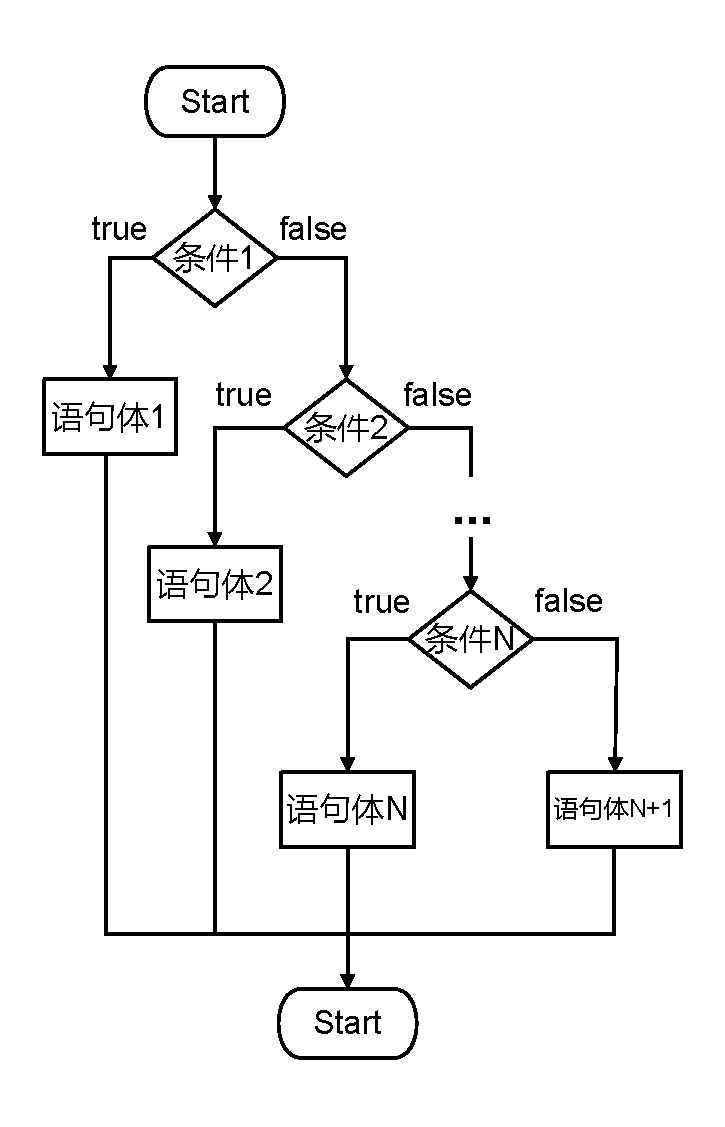
\includegraphics[width=0.5\textwidth]{pictures/switch结构.pdf}
	\caption{switch结构}
	\label{fig:switch结构}
\end{figure}

图\ref{fig:switch结构}是switch语句的程序控制流图。
图4-11是 switch 语句的程序控制流图。根据 C语言 的语义,switch 语句首先计算控制表达式的值。然后,该值与 case 标签所指定的值进行比较。如果找到与控制表达式的值匹配的 case 标签,程序将从该 case 标签开始执行对应的语句,执行完毕后,程序将继续匹配下一个case标签。如果没有匹配的 case 标签,且存在 default 标签,那么程序将执行 default 标签处的语句;如果没有 default 标签,则 switch 语句执行结束而不执行任何语句。

在 switch 语句中,break 语句需要特殊处理,continue语句则不需要:当 case 或 default 语句块中遇到 break 语句时,程序将跳出 switch 语句的执行。因此,在为 switch 语句的case生成 NFA 时,工具原型应该将 switch 语句的出口作为case中的 break 语句的跳转目标(breakTgt),将 switch 语句
上一层次的语句自动机中记录的 continue语句的跳转目标(continueTgt)直接继承给 case 语句,作为 case 语句中的 continue 语句的跳转目标。即工具原型在case内部处理 break 语句时,需要将该 break 语句对应的自动机的出口连接到 switch 语句自动机的出口;
在case中的 continue 语句时,需要将 continue 语句的自动机的出口连
接到上一层次的语句自动机的 continueTgt。

 \begin{figure}[htbp]
	\centering
\begin{minipage}{16cm}
\begin{lstlisting}
buildAutomaton(breakTgt,continueTgt): 
    #对switch结构的处理
    获取包含多个case的复合语句的AST节点cases
    casesAutomaton = Automaton()        #为cases初始化一个Automaton类的对象
    casesAutomaton.buildAutomaton(cases,breakTgt=self.end_state,continueTgt,self.continueTgt)    
    #构造cases的自动机casesAutomaton
    按照程序控制流图,将swich语句中不同部分的自动机连接起来
    ... ...
    #对单个case结构的处理
    获取condition的AST节点cond,并构造生成condition的自动机condAutomaton
    获 取statements的AST节点stmts
    stmtsAutomaton = Automaton(); #为statements初始化一个Automaton类的对象
    stmtsAutomaton.buildAutomaton(stmts,breakTgt=cases.breakTgt,continueTgt=cases.continueTgt)     
    #构造statements的自动机stmtsAutomaton
    按照程序控制流图,将单个case语句中不同部分的自动机连接起来
\end{lstlisting}   
\end{minipage}
    \caption{对switch结构和单个case结构的处理}
    \label{对switch结构和单个case结构的处理}
\end{figure}

图\ref{对switch结构和单个case结构的处理}是对switch结构和单个case结构的处理的伪代码。
工具原型将先获取switch语句中的包含多个case的复合语句的AST节点cases, 为cases初始化一个 Automaton 类的对象 casesAutomaton,
并设置 breakTgt和 continueTgt,最后调用buildAutomaton方法递归生成casesAutomaton的不确定自动机。
因为cases的AST节点的类型为“COMPOUND\_STMT”,buildAutomaton方法将会把case节点视为复合语句节点,以处理顺序结构的方式处理cases节点,按照程序控制流图,将cases内的每个case按照顺序连接:
\begin{itemize}
    \item switch语句的自动机的入口连接到casesAutomaton的入口;
    \item casesAutomaton内的每一个case自动机(caseAutomaton)将依次首尾相连;
    \item casesAutomaton的出口将连接上switch语句的自动机的出口。
\end{itemize}

此外,工具原型还实现了对于单个case语句的处理。工具原型将先获取case语句中的condition的AST节点cond和statements的AST节点stmts。然后为条件表达式cond生成自动机condAutomaton(它是Automaton类的一个对象);同时为stmts初始化一个Automaton类的对象stmtsAutomaton,并继承switch自动机本身的breakTgt和continueTgt,最后调用buildAutomaton方法递归生成stmtsAutomaton的不确定自动机。最后按照程序控制流图,将case语句中不同部分的自动机连接起来,生成caseAutomaton:
\begin{itemize}
    \item case语句的自动机的入口连接到condAutomaton的入口;
    \item condAutomaton的出口将以“True”的标签连接到stmtsAutomaton的入口,同时以“False”的标签连接到case语句的自动机的出口;
    \item stmtsAutomaton的出口将连接上case语句的自动机的出口。
\end{itemize}



\subsection{从初始NFA获取日志函数的输入,最终生成DFA的方法}
当工具原型得到由自动机组成的初始NFA后,还需要对其进一步处理。
因为待分析的日志记录中只有日志函数的输出,所以,需要保证自动机的边上的输入只能来自log日志函数的参数。
因此,工具原型先将无用的标签去掉,使得初始的NFA转为只有合法输入的NFA。
在这种情况下,所有没有标签的边在新的NFA中都被当做空边处理。

接下来,为了实现子集构造法,工具原型实现了一个返回状态的空边闭包的函数

图\ref{返回状态的空边闭包}的函数将返回给定集合的epsilon闭包。\\
 \begin{figure}[htbp]
	\centering
\begin{minipage}{14cm}
\begin{lstlisting}
epsilon_closure(states):
    初始化closure,queue
    当queue不为空时:
        current_state = queue.pop()
        将epsilon_transitions设为从current_state出发的所有空边的目的地
        对于epsilon_transitions中每一个state:
            if state 不在 closure内:
                将state加入queue和closure
    return frozenset(closure)
\end{lstlisting}
    \caption{返回状态的空边闭包}
    \label{返回状态的空边闭包}
\end{minipage}
\end{figure}
这段代码是一个函数epsilon\_closure,它接收一个状态集合作为输入参数。
它的功能是计算从给定的状态集合出发,通过空边可以到达的所有状态,然后返回这些状态的闭包。
代码的执行过程如下:
首先,将输入的状态集合初始化为闭包集合closure,同时将该集合添加到一个队列queue中。
进入循环,只要队列不为空,就执行以下操作:
\begin{itemize}
	\item 弹出队列中的一个状态current\_state作为当前状态。
	\item 找到从当前状态出发的所有空边的目的地,这些目的地的标签为空。将这些目的地添加到列表epsilon\_transitions中,其中列表元素是状态。
	\item 对于每个目的地状态state,如果它不在闭包集合closure中,就将它添加到闭包集合中,并将其加入队列queue中,以便后续继续扩展闭包。
\end{itemize}

循环结束后,闭包集合closure中包含了从输入状态集合出发,通过空边可以到达的所有状态。最后
使用frozenset将其转换成不可变的冻结集合,并作为结果返回。

接下来,工具原型实现了一个NFA到DFA的转换函数(图\ref{子集构造法}),并在其中调用了图\ref{返回状态的空边闭包}的epsilon\_closure函数。

 \begin{figure}[htbp]
	\centering
\begin{minipage}{16cm}
\begin{lstlisting}
NFA2DFA(self):
    将初始的unmarked_states设为main函数的startNode的epsilon闭包
    获取自动机的字符表alphabet
    当 unmarked_states 不为空时:
        current_states = unmarked_states.pop(0)
        对于alphabet中的每一个symbol:
            next_states = set()
            对于current_states中的每一个state:
                寻找通过symbol可以到达的state,并将其epsilon闭包加入next_states
            if next_states不为空:
                if next_state不在DFA中
                    将next_states加入DFA
                    将next_states加入unmarked_states
                连接current_states到next_state,标签为symbol
\end{lstlisting}
\end{minipage}
    \caption{子集构造法}
    \label{子集构造法}
\end{figure}
首先,从NFA的起始状态集合(设定为main函数的入口)开始,使用epsilon\_closure函数计算该状态集合的epsilon闭包,
并将其作为初始状态加入DFA中。
创建一个列表unmarked\_states,用于存储未标记的DFA状态集合(即待处理的状态集合)。
只要unmarked\_states不为空,就循环执行以下操作:
\begin{enumerate}
	\item 弹出unmarked\_states列表的第一个元素(DFA的state),加入当前状态集合current\_states。
	\item  对于输入字符集合中的每个输入符号symbol(也就是日志记录文件中的一条记录),创建一个空集合next\_states,
 用于存储当前状态集合通过
 symbol转换能够到达的状态集合,对于current\_states中的每个状态state,
 找到从state经过symbol转换可以到达的状态集合transitions。
 对于transition\_state中的每个状态,
 计算其epsilon闭包,并将这些状态添加到next\_states集合中。
	\item 如果next\_states非空,则将
 next\_states作为新的DFA状态集合next\_state。
 如果next\_state尚未添加到DFA中,则将其添加为一个新的状态,
 并将其添加到unmarked\_states列表中,以进行后续处理。
 在DFA中添加一条边,从current\_states到next\_state,标记为symbol。
\end{enumerate}
循环结束后,DFA的构建完成,其中每个节点表示一个DFA状态集合,边表示状态之间的转换,标记为输入符号。
\subsection{结合DFA,解析日志序列}
最后一步,工具原型实现了函数runDFA,它可用生成的DFA,解析日志记录。

图\ref{以日志为输入,运行DFA}函数将用DFA解析给定的日志记录,若结果错误(输入不合法或者日志错误),将返回一个空的列表;
否则,返回源程序在运行时,经过的DFA的stateNode的一个列表,这在一定程度上表示了程序的运行路径。\\
 \begin{figure}[htbp]
	\centering
\begin{minipage}{8cm}
\begin{lstlisting}
runDFA(self):
    读取输入文件
    输入字符的合法性检查
    初始化 DFA 的状态 current_state
    维护一个 visited_states 列表
    运行状态转移
    返回走过的state列表,用于后续染色展示
\end{lstlisting}
\end{minipage}
    \caption{以日志为输入,运行DFA}
    \label{以日志为输入,运行DFA}
\end{figure}

首先,这个函数将打开一个名为 loginfo.txt 的文件,
作者假设需要分析的日志就在其中。函数将去除每行的换行符和空白字符,
并读取其中的所有行。接着工具原型将检查每个处理后的字符是否在 DFA 的输入字符集合中,
如果不在,打印错误信息并返回空列表。

其次,将current\_state首先设置为 DFA 的开始状态
(其中必定包含NFA中的main函数的startNode节点)。
将current\_state加入visited\_states的list,
用于记录DFA运行时访问过的所有节点。

对于日志记录中每一行的日志log,工具原型将其看作自动机的一个输入字符,并在当前状态的所有转移边中寻找匹配的边。
检查当前状态的每一条转移边的标签是否与当前输入字符匹配。
如果找到匹配的边,更新 current\_state 为下一个状态,
并将其添加到 visited\_states 中。
如果没有找到匹配的转移边,说明日志记录错误(不可能存在这样的日志序列),打印错误信息并返回空列表。

最后,如果所有输入字符都合法且找到对应的状态转移,
返回运行时访问过的所有节点的列表 visited\_states,工具原型将会把存在于visited\_states中的状态节点染上不同颜色,用于区分展示。\\

在得到了所有日志相关的信息后,工具原型便可对工具原型的运行情况进行进一步的分析。

如果自动机成功运行到了接受状态,工具原型可以根据生成的DFA(如图\ref{fig:日志分析的可视化}),了解它的实际运行过程,比如经过了哪些语句,在选择语句时选择了哪一个分支等等。

如果自动机没有运行到接受状态,而是停在了中间的某个位置,开发人员便可针对
这类情况设计特殊的日志,进行错误分析,以及出错时调用栈的内容。
\begin{enumerate}
    \item 识别错误日志记录:假设每条记录的格式已知,
    并且包含明确的错误标识符(例如,"ERROR"、"EXCEPTION" 等),
    开发人员可以扫描日志内容,找出所有包含这些关键字的日志,进而分析程序的错误是如何生成的。
    \item 解析程序点的位置:假设日志记录中包含有关程序点的信息,如函数名、文件名和行号。
    这些信息通常在错误日志中出现,开发人员可以通过解析错误发生时周围的日志来找到。
    \item 提取错误发生时的调用栈内容:假设开发人员在每个函数的入口处和出口都放置一条
    日志函数代表该函数的调用和退出,这样在程序发生错误后,这些信息会详细列出错误发生时的函数调用顺序,
    开发人员便可以用这类日志函数来判断函数发生错误时的调用栈。
\end{enumerate}

\section{本章小结}
本章深入到工具原型实现的细节,涵盖了工具原型的运行环境配置、关键功能的实现步骤和具体技术细节。

在工具原型运行环境部分,工具原型使用Python 3.10.8作为开发和运行的编程语言,
并安装Clang 12.0.0及其Python绑定模块Clang.cindex。
此外,还需要安装Python库NetworkX用于处理自动机组成的有向图网络。

关键功能实现部分描述了工具原型的核心功能,分为四个主要步骤:
\begin{enumerate}
    \item 从C语言程序生成抽象语法树(AST)。
    \item 递归解析AST,生成初步的非确定有限自动机(NFA)。
    \item 根据NFA获取日志信息,进一步生成确定有限自动机(DFA)。
    \item 结合DFA,解析日志序列。
\end{enumerate}

每个步骤都有详细的伪代码片段和解释,
例如从C语言程序生成AST的过程使用了Clang的接口和Python代码示例,
展示了如何处理不同类型的AST节点来构建NFA。
递归解析AST的过程中,通过Automaton类表示自动机,
并展示了如何处理不同的语句结构(如顺序结构、循环结构、条件结构等)
以及函数调用和控制流语句。

最后,文章描述了从初始NFA获取日志信息并生成DFA的过程,
涉及到epsilon闭包的计算和子集构造法的应用,
以确保工具原型能够准确解析和识别特定的日志信息。



\chapter{系统测试}
\section{测试目的}
\section{测试内容}
\section{测试方法}






%---------------------------------------------------------------------
%	参考文献
%---------------------------------------------------------------------

% 生成参考文献页
\printbibliography

%---------------------------------------------------------------------
%	致谢
%---------------------------------------------------------------------

\begin{acknowledgement}

\end{acknowledgement}

%---------------------------------------------------------------------
%	学术简历
%---------------------------------------------------------------------

% 详见手册中“成果列表”一节
% \njuchapter{学术成果}
% \njupaperlist[攻读博士学位期间发表的学术论文]{preskill2018}

%---------------------------------------------------------------------
%	附录部分
%---------------------------------------------------------------------

% 附录部分使用单独的字母序号
%\appendix

% 可以在这里插入补充材料
%\chapter{正文中涉及的数据及源代码}
%\dots

% 完工
\end{document}
